\documentclass{article}

% if you need to pass options to natbib, use, e.g.:
%     \PassOptionsToPackage{numbers, compress}{natbib}
% before loading neurips_2026

% The authors should use one of these tracks.
% Before accepting by the NeurIPS conference, select one of the options below.
% 0. "default" for submission
% \usepackage{neurips_2026}
% the "default" option is equal to the "main" option, which is used for the Main Track with double-blind reviewing.
% 1. "main" option is used for the Main Track
%  \usepackage[main]{neurips_2026}
% 2. "position" option is used for the Position Paper Track
%  \usepackage[position]{neurips_2026}
% 3. "eandd" option is used for the Evaluations & Datasets Track
 % \usepackage[eandd]{neurips_2026}
% 4. "creativeai" option is used for the Creative AI Track
%  \usepackage[creativeai]{neurips_2026}
% 5. "sglblindworkshop" option is used for the Workshop with single-blind reviewing
 % \usepackage[sglblindworkshop]{neurips_2026}
% 6. "dblblindworkshop" option is used for the Workshop with double-blind reviewing
%  \usepackage[dblblindworkshop]{neurips_2026}

% After being accepted, the authors should add "final" behind the track to compile a camera-ready version.
% 1. Main Track
 % \usepackage[main, final]{neurips_2026}
% 2. Position Paper Track
%  \usepackage[position, final]{neurips_2026}
% 3. Evaluations & Datasets Track
 % \usepackage[eandd, final]{neurips_2026}
% 4. Creative AI Track
%  \usepackage[creativeai, final]{neurips_2026}
% 5. Workshop with single-blind reviewing
%  \usepackage[sglblindworkshop, final]{neurips_2026}
% 6. Workshop with double-blind reviewing
%  \usepackage[dblblindworkshop, final]{neurips_2026}
% Note. For the workshop paper template, both \title{} and \workshoptitle{} are required, with the former indicating the paper title shown in the title and the latter indicating the workshop title displayed in the footnote.
% For workshops (5., 6.), the authors should add the name of the workshop, "\workshoptitle" command is used to set the workshop title.
% \workshoptitle{WORKSHOP TITLE}

% "preprint" option is used for arXiv or other preprint submissions
\usepackage[preprint]{neurips_2026}
\setcitestyle{round,aysep={}}

% to avoid loading the natbib package, add option nonatbib:
%    \usepackage[nonatbib]{neurips_2026}

\usepackage[utf8]{inputenc} % allow utf-8 input
\usepackage[T1]{fontenc}    % use 8-bit T1 fonts
\usepackage{hyperref}       % hyperlinks
\usepackage{url}            % simple URL typesetting
\usepackage{booktabs}       % professional-quality tables
\usepackage{amsfonts}       % blackboard math symbols
\usepackage{nicefrac}       % compact symbols for 1/2, etc.
\usepackage{microtype}      % microtypography
\usepackage{minted}       % python code
\usepackage{xcolor}         % colors
\usepackage{graphicx}       % \resizebox for scaling figures to column width
\usepackage{amsmath}        % for \tfrac
\usepackage{tikz}
\usetikzlibrary{positioning, arrows.meta, shapes.geometric}
\usetikzlibrary{positioning, arrows.meta}
\usepackage{color, soul}    % highlighting during editing
% figure palette (semantic colors shared by all TikZ diagrams)
\colorlet{featuregroup}{blue!15}          % Feature Group / Concept Instance fill
\colorlet{feature}{black!10}              % Feature color
\colorlet{context}{red!15}                % Context fill
\colorlet{transform}{yellow!30}           % Transform fill
\definecolor{transformedge}{HTML}{9900CC} % Transform (dashed) edges
\colorlet{delta}{black!10}                % Delta fill
\colorlet{concept}{green!15}              % Concept fill
\colorlet{conceptedge}{green!55!black}    % Concept link lines
\colorlet{valence}{teal!25}               % Valence fill
\colorlet{action}{orange!25}              % Action fill

% code style
\setminted[python]{
    frame=lines,
    framesep=2mm,
    baselinestretch=1.2,
    bgcolor=lightgray!20,
    fontsize=\footnotesize,
    linenos
}

% Note. For the workshop paper template, both \title{} and \workshoptitle{} are required, with the former indicating the paper title shown in the title and the latter indicating the workshop title displayed in the footnote. 
\title{Emergent Ontologies for Continuous Online Learning}


% The \author macro works with any number of authors. There are two commands
% used to separate the names and addresses of multiple authors: \And and \AND.
%
% Using \And between authors leaves it to LaTeX to determine where to break the
% lines. Using \AND forces a line break at that point. So, if LaTeX puts 3 of 4
% authors names on the first line, and the last on the second line, try using
% \AND instead of \And before the third author name.


\author{%
  Adam Powers \\
  El Dorado Hills, CA 95762 \\
  \texttt{apowers@ato.ms} \\
  % examples of more authors
  % \And
  % Coauthor \\
  % Affiliation \\
  % Address \\
  % \texttt{email} \\
  % \AND
  % Coauthor \\
  % Affiliation \\
  % Address \\
  % \texttt{email} \\
  % \And
  % Coauthor \\
  % Affiliation \\
  % Address \\
  % \texttt{email} \\
  % \And
  % Coauthor \\
  % Affiliation \\
  % Address \\
  % \texttt{email} \\
}

\begin{document}


\maketitle


\begin{abstract}
  % TODO
  TODO
\end{abstract}



\section{Introduction}
There is growing recognition that AI systems need structured world knowledge -- representations that support not just pattern matching but prediction, planning, reasoning, and transfer. Recent research in world models \hl{...}, neurosymbolics \hl{...}

Disposition of problem and existing work \hl{...}
\hl{**FEP / predictive coding:** Friston (2010; 2006); Rao \& Ballard (1999); Knill \& Pouget (2004); Friston, *Predictive coding under the free-energy principle*, 2009; FEP precision/neuromodulation literature, e.g. cholinergic-modulation PMC4235126}

In this paper we propose a cognitive architecture that is a synthesis of existing research. The architecture creates a graph-based world model that we refer to as an ontology. The ontology is created from perceptions of the environment in the same spirit as Barsalou's Perceptual Symbol Systems \citep{Barsalou_1999}. The ontology does not use first order logic for edges / relationships, but probabilistic links that approximate Friston's Free Energy Principle \citep{friston_free_2006}. The ontology is formed through one-shot acquisition, and probabilistic relationships are sculpted over time to provide higher confidence about the environment.

The foundational principles of the architecture are:
\begin{itemize}
    \item Symbols (referred to as Concepts) are required for transfactuality and one-shot learning
    \item Concepts and predictions are acquired on first encounter, confidence and precision is sculpted over time
    \item Concepts are the locus of transfactuality and prediction (as opposed to many reinforcement learning systems where states are the locus of transfactuality)
    \item Predictions must be context specific; depending on which concepts are currently present, predictions will be different
    \item Must be able to remember specific instances (where did I leave my keys) independent from generalities
    \item Concepts are assumed to be true, and truer the more they are predictively accurate, until a new experience proves otherwise. This "bold prediction" is enabled by graph structure, not probability.
    \item The structure of the ontology is emergent and stratified. There is no presupposed hierarchy, classes, or relationships. All are learned and path-specific.
    \item Prediction primacy, reward secondary (based on latent learning and sparse rewards)
    \item The goal of the system is to provide accurate predictions for homeostasis and simulation to resolve sensory valance issues that arise from time to time.
    \item Feature extractors and saliency reduce the environment to a tractable, structured space
    \item Perceptual grounding with a minimal innate endowment
    \item Must be computationally plausible on commercially available hardware in near real-time (seconds, subsecond), even if it requires high parallelism. This is to focus our work on practical solutions rather than pure theoretical approaches.
    \item The system is built out of a minimal number of mechanisms
\end{itemize}

We argue that the capacity for one continual unsupervised online learning — acquiring and immediately using new world knowledge from single experiences — does not require scale, supervision, or hand-engineered ontologies, but follows naturally when concepts are allowed to emerge bottom-up as a stratified graph structure built directly from perceptual features and sensory valence signals. We position this as a viable and underexplored alternative to the dominant approaches: large-corpus learning, world models, symbolic knowledge engineering, and prior cognitive architectures.

```
this paper makes two falsifiable predictions:

**PRIMARY 1 — Generalization/accuracy dissociation (learning is USEFUL).** After single-exposure acquisition, **accuracy on already-seen instances saturates quickly** while **generality to novel same-concept instances keeps rising** over repetitions — the two curves visibly *separate*.
- *Why it's the fingerprint of the core claim:* the theory's defining assertion is that acquisition and generalization are **separate processes at separate rates**. This signature separates the two processes *in the data* and shows they move independently. Pure-incremental (one mechanism) moves accuracy and generality *together* -> no separation. Pure-one-shot -> both flat after exposure 1. **Only a two-process system shows the separation.** If they rise together, the two-timescale claim is wrong.
- *Operationalization:* performance on repeated instances (accuracy) vs held-out novel same-concept instances (generality), over exposure count. Requires a domain where "same concept, novel instance" is generable. **Experiment: transfer across multiple gyms** (user) — a transform learned in one gym firing correctly in new gyms exercises this directly.

**PRIMARY 2 — Convergence / "knitting" (learning is STABLE).** The acquisition+sculpting of all four parts (concepts, contexts, transforms, features) must knit to a **stable functional structure, not an unusable mess**. Measurable sub-claim
**Prediction-error decline:** average precision-weighted error falls and **plateaus**, not oscillates. *Falsifier:* sustained oscillation = the acquire/sculpt loop thrashing (spawn/forget the same structures) = the "unusable mess."
- *Why co-primary, not a footnote:* it tests a **different axis** than PRIMARY 1 — usefulness vs stability, which fail *independently* (a system can converge to a stable-but-useless model, or generalize transiently while never stabilizing). And unbounded structural churn is the *characteristic* failure a critic would predict of a bold-projection + easy-spawn architecture, so demonstrating convergence directly answers the strongest objection and directly tests closed loop converges; open loop churns.
```

Not a single new mechanism but a synthesis. \hl{...}

The rest of the paper is organized as follows. \hl{...}

\section{Positioning Versus Other Approaches}
- vs. LLMs / deep learning: enables one-shot / few-shot learning from experience; does not require massive training datasets or millions of cycles
- vs. manual knowledge engineering (Cyc, OO-MDP): concepts are learned bottom-up from perception and valence signals, not hand-crafted by engineers
- vs. formal logic systems (Cyc): does not require first-order logic representations; concepts are grounded in perception
- vs. traditional RL: interposes a conceptual layer that enables transfer, abstraction, and planning beyond raw state-action mappings
- [?] Position against other cognitive architectures (ACT-R, SOAR, CLARION)?

\section{Knitting: Formation of Data Structures}
At the core is creating data structures that can be used for understanding, navigating, and manipulating the world -- especially one-shot, online learning. Environmental features and reinforcement signals are turned into concepts and temporal timelines that can be used to model the world, predict action outcomes, and simulate the environment. These concepts and temporal timelines are emergent and stratified and created from the environment itself; they are not \emph{a priori}.

One of the largest challenges with creating a world representation using data is the cold start problem -- how is the agent productive when little or no initial data is available. Therefore, the sections below are presented in the order of bootstrapping the system, putting aside the optimizations and additional benefits of having access to established concepts.

\subsection{Sensory Input, Feature Extraction, Saliency}
This section lays out the basic units for forming concepts. Concepts are initially built from features, bound together at a specific space and time by their co-occurrenced. The mechanisms described in this section are well established both biologically and algorithmically and assumed to be non-controversial; however, the novel contribution is the shape of the data at the end of the feature extraction process that will be used as the basis for formulating and using concepts.

In order for the agent to reduce the data received from the environment to a manageable stream of information, multisensory input is initially broken down into a series of features using modality-specific feature extractors: edges, lines, vertices, colors, gradients, motion, in vision; frequency, harmonicity in the auditory system; edges, points, curvature, vibration in haptics; and so forth. Extracted features may be compounded to create increasingly complex features, such as creating 'T' or 'L' shape feature detectors from a combination of lines detected by the visual system. Each of these becomes a standalone feature -- an atomic node that will be used to create concepts. The modality, quantity, and types of feature extractors is not central to this argument. It is sufficient to say that there are a large number of them and the more that are available, the better the agent will be at creating differentiated concepts. It is also important to note that there are a fixed number of types of concepts: the set of types of features that can be generated by the agent is determined by number and types of feature extractors. \citep{pashler_attention_2016} \hl{other citations}

Each feature is mapped to a specific location in space, relative to the agent. The dimensionality of the space is unimportant, only that features can be colocated at a specific point in time so that they can be bound together. Modality-specific saliency mechanisms \hl{Itti and Koch; Auditory saliency} (such as brightness, loudness, or motion) are used to select candidate feature groups, inhibition of return \hl{citation} is applied to ensure the agent does not become locked to a single salient point to the exclusion of all others, and cross-modal attention selects which features receive bottom-up attention using a winner-take-all mechanism. For the moment, we will put aside other context-specific mechanisms that may modify the selection of feature groups from the environment, such as agentic context that influences the selection of features. The winning features are bound together based on their spatiotemporal locus to create a FeatureGroup \citep{Kahneman_Treisman_Gibbs_1992, pylyshyn_role_1989, Wolfe_2021, treisman_binding_1996} \hl {TODO citation Feature binding, attention and object perception}. This FeatureGroup plays the role of the physical instance of a Concept, as we will note later. Note that only the features at that location are bound together, meaning that not all features are present in the FeatureGroup. The result of the feature extraction and saliency processes a sequential stream of feature groups at specific spatiotemporal locations. In our system, this information will be represented as a graph: a Feature Group node, with edges describing the features that create the composition of the features at that point in time.

- These FeatureGroups are important because a single concept may be present multiple times at the same time. If I am holding three marbles, they all have the same concept / predictive capability, even though there are three distinct objects.

\begin{figure}[ht]
  \centering
  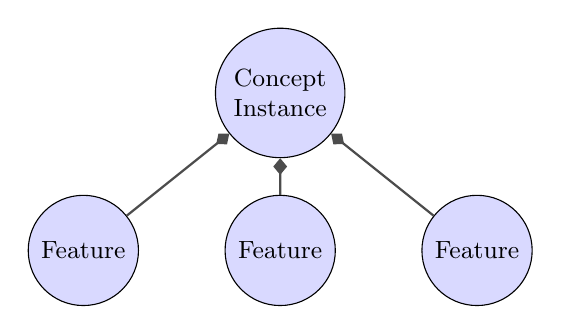
\begin{tikzpicture}[
    every node/.style={circle, draw, fill=featuregroup, minimum size=1.4cm, font=\small, align=center},
    edge from parent/.style={draw, {Diamond[length=6pt, width=5pt]}-, thick, color=black!70},
    level 1/.style={sibling distance=2.5cm, level distance=2cm}
  ]
    \node {Concept\\Instance}
      child {node {Feature}}
      child {node {Feature}}
      child {node {Feature}};
  \end{tikzpicture}
  \caption{A concept instance binds together the features detected at a spatiotemporal locus.}
  \label{fig:concept-instance}
\end{figure}

\subsection{Context: Point in Time Relationships}
As this stream of feature groups is created, all pairwise relationships are defined within some window of time along multiple dimensions. For example, depending on the agent, the window of time may be seconds or milliseconds where all the feature groups are connected by relationships of distance, change in distance, orientation, and change in orientation in egocentric and allocentric frames of reference \citep{Hafri_Firestone_2021,vo_reading_2019}.

These relationships are used to construct mereotopological types of concepts (e.g. part of, connected to, separate from) as well as concepts used for reasoning about relationships between disjointed objects (e.g. getting closer, touching). The collection of relationships between these Concepts at a specific point in time create Contexts, which can be used to encode specific points of time in episodic memory -- the set of features that was perceived at a specific point in time and the relation to each other, in such a way that a point in time can be reconstructed (albeit in a lossy manner). This also holds future utility in identifying and reusing instance data -- contexts can be used to identify similar situations that have occurred before.

Note that our definition of the term Context here differs from the everyday usage of the term -- our Contexts are at a much finer grain where every change in the Concepts present or the relationships between them creates an entirely new Context. As foreshadowing to future sections, the reason that Contexts are created when relationships change is that relationships are critical for prediction: the presence of the "fire" Concept in a Context has completely different predictive capabilities based on whether it is far (just a light source), near (a warm heat source), touching (painful sensory valence), below (hotter since heat rises), or above (colder since the heat is rising). Over time, as Abstraction (see Section \ref{sec:abstraction}) creates high-level Concepts such as "stove" and "refrigerator", Concepts may also be abstracted to carry the same meaning as their every-day usage such as "kitchen"; however, that presumes multiple iterations of successful Abstraction for both Concepts and Contexts over long periods of time.

\begin{figure}[ht]
  \centering
  \resizebox{\linewidth}{!}{%
  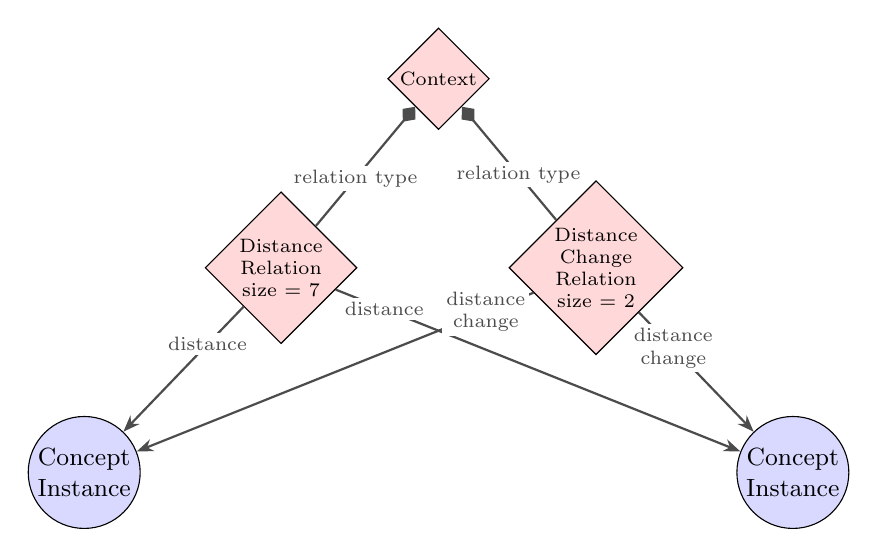
\begin{tikzpicture}[
    circ/.style={circle, draw, fill=featuregroup, minimum size=1.4cm, font=\small, align=center, inner sep=1pt},
    rel/.style={diamond, draw, fill=context, font=\scriptsize, align=center, inner sep=1pt},
    agg/.style={{Diamond[length=7pt, width=6pt]}-, thick, color=black!70},
    assoc/.style={-{Stealth[length=6pt]}, thick, color=black!70},
    lbl/.style={font=\scriptsize, fill=white, inner sep=1.5pt, align=center},
    x=1cm, y=1cm
  ]
    % concept instances (bottom row)
    \node[circ] (ciL) at (0,0) {Concept\\Instance};
    \node[circ] (ciR) at (9,0) {Concept\\Instance};
    % relation types
    \node[rel] (dr)  at (2.5,2.6) {Distance\\Relation\\size = 7};
    \node[rel] (dcr) at (6.5,2.6) {Distance\\Change\\Relation\\size = 2};
    % context
    \node[rel] (rg) at (4.5,5.0) {Context};

    % association: each relation type relates the two concept instances
    \draw[assoc] (dr)  -- (ciL) node[lbl, pos=0.30] {distance};
    \draw[assoc] (dr)  -- (ciR) node[lbl, pos=0.12] {distance};
    \draw[assoc] (dcr) -- (ciL) node[lbl, pos=0.12] {distance\\change};
    \draw[assoc] (dcr) -- (ciR) node[lbl, pos=0.30] {distance\\change};

    % aggregation: the context is composed of its relation types
    \draw[agg] (rg) -- (dr)  node[lbl, pos=0.6] {relation type};
    \draw[agg] (rg) -- (dcr) node[lbl, pos=0.6] {relation type};
  \end{tikzpicture}%
  }
  \caption{A Context captures the pairwise relationships -- such as distance and change in distance -- between concept instances at a single point in time. Each relation type relates the concept instances it connects. (The features associated with the concept instances have been omitted for clarity.)}
  \label{fig:context}
\end{figure}

\subsection{Episodic Timeline}\label{sec:episodic-timeline}
Whereas the Contexts are a point-in-time snapshot of the environment, the Episodic Timeline is a series of relationships between Contexts to create a dynamic, ongoing view of the environment and its changes. The Episodic Timeline and its Transforms are the foundation for one-shot online learning. They are the view of the ontology graph that describes what happened (or is happening) in terms of specific instances of concepts and point-in-time changes. It is also a recording of what has happened so that it can be used in future predictions. This timeline is not created at regular time intervals, but at the cadence that new relationships are created, which is dictated by salience; the relationships are merely before / after, not a specific amount of time before or after.

This system links Feature Groups across Contexts, identifying the same or similar feature groups in successive Contexts. This similarity is aided by feature extractors that detect motion, which reduces the dependence on similarity for tracking feature groups over time \citep{kalal_tracking-learning-detection_2012}. Each FeatureGroup that is determined to be the same across multiple steps in the Episodic Timeline is linked back to a Concept node in the graph. The system also creates transforms between each successive Feature Group, indicating how the Feature Group or Relationship Group changed at different points in time. 

The content of Transforms corresponds to the types of features generated by the feature extractors and the types of relationships between objects. Each Transform carries one or more Features (e.g. color, lines, intersections, gradient size) or Relationships (e.g. distance, orientation) that has changed between successive steps. Only changes are recorded in the transform and they are encoded as differences between values or states. For an example of a red hue from 100 to 150 would be ncoded as "red: +50" in the transform. This enables transforms to be applied in future scenarios as a prediction of what will happen -- the same Concept in the same Context would be expected to add +50 to its red hue. See Section \ref{pseudocode:transforms} for a more detailed specification of the content of Transforms.

\begin{figure}[ht]
  \centering
  \resizebox{\linewidth}{!}{%
  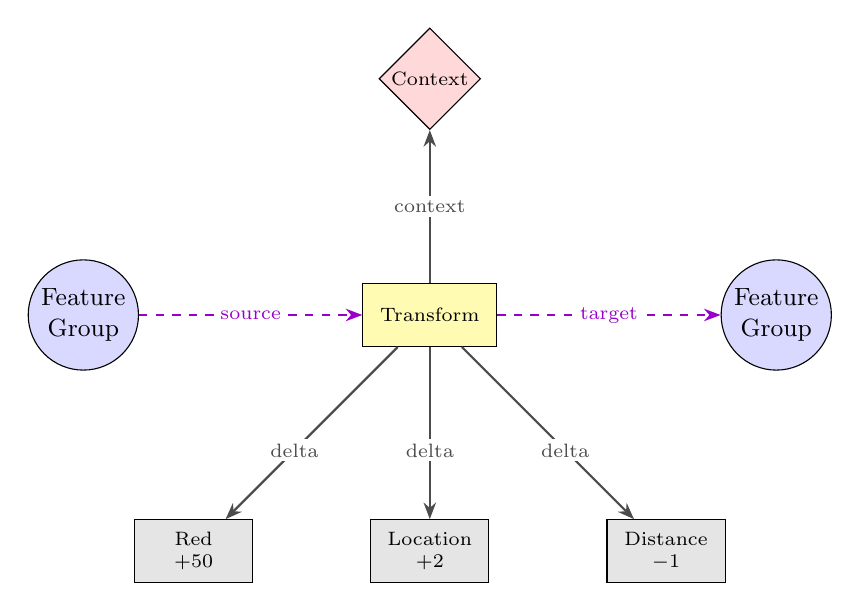
\begin{tikzpicture}[
    circ/.style={circle, draw, fill=featuregroup, minimum size=1.4cm, font=\small, align=center, inner sep=1pt},
    rel/.style={diamond, draw, fill=context, font=\scriptsize, align=center, inner sep=1pt},
    trans/.style={rectangle, draw, fill=transform, font=\scriptsize, align=center, inner sep=3pt, minimum height=0.8cm, minimum width=1.7cm},
    delta/.style={rectangle, draw, fill=delta, font=\scriptsize, align=center, inner sep=3pt, minimum height=0.8cm, minimum width=1.5cm},
    assoc/.style={-{Stealth[length=6pt]}, thick, color=black!70},
    tedge/.style={-{Stealth[length=6pt]}, thick, dashed, color=transformedge},
    lbl/.style={font=\scriptsize, fill=white, inner sep=1.5pt, align=center},
    x=1cm, y=1cm
  ]
    % feature groups (middle row) and the transform between them
    \node[circ]  (fgs) at (0,0)   {Feature\\Group};
    \node[trans] (t)   at (4.4,0) {Transform};
    \node[circ]  (fgt) at (8.8,0) {Feature\\Group};

    % context (above the transform)
    \node[rel] (ctx) at (4.4,3.0) {Context};

    % deltas (below the transform)
    \node[delta] (d1) at (1.4,-3.0) {Red\\+50};
    \node[delta] (d2) at (4.4,-3.0) {Location\\+2};
    \node[delta] (d3) at (7.4,-3.0) {Distance\\$-1$};

    % transform edges: source Feature Group -> Transform -> target Feature Group
    \draw[tedge] (fgs) -- (t)   node[lbl, pos=0.5] {source};
    \draw[tedge] (t)   -- (fgt) node[lbl, pos=0.5] {target};

    % the transform is recorded in a context
    \draw[assoc] (t) -- (ctx) node[lbl, pos=0.5] {context};

    % the transform carries its deltas
    \draw[assoc] (t) -- (d1) node[lbl, pos=0.6] {delta};
    \draw[assoc] (t) -- (d2) node[lbl, pos=0.6] {delta};
    \draw[assoc] (t) -- (d3) node[lbl, pos=0.6] {delta};
  \end{tikzpicture}%
  }
  \caption{Transform nodes are between FeatureGroups and capture the change between two FeatureGroups in a specific Context. They are created between each tick of the agent and capture the changes in the FeatureGroup between ticks as Deltas. The Transforms can later be applied when the same or similar Context is encountered to predict the next Context.}
  \label{fig:transform}
\end{figure}

\begin{figure}[ht]
  \centering
  \resizebox{\linewidth}{!}{%
  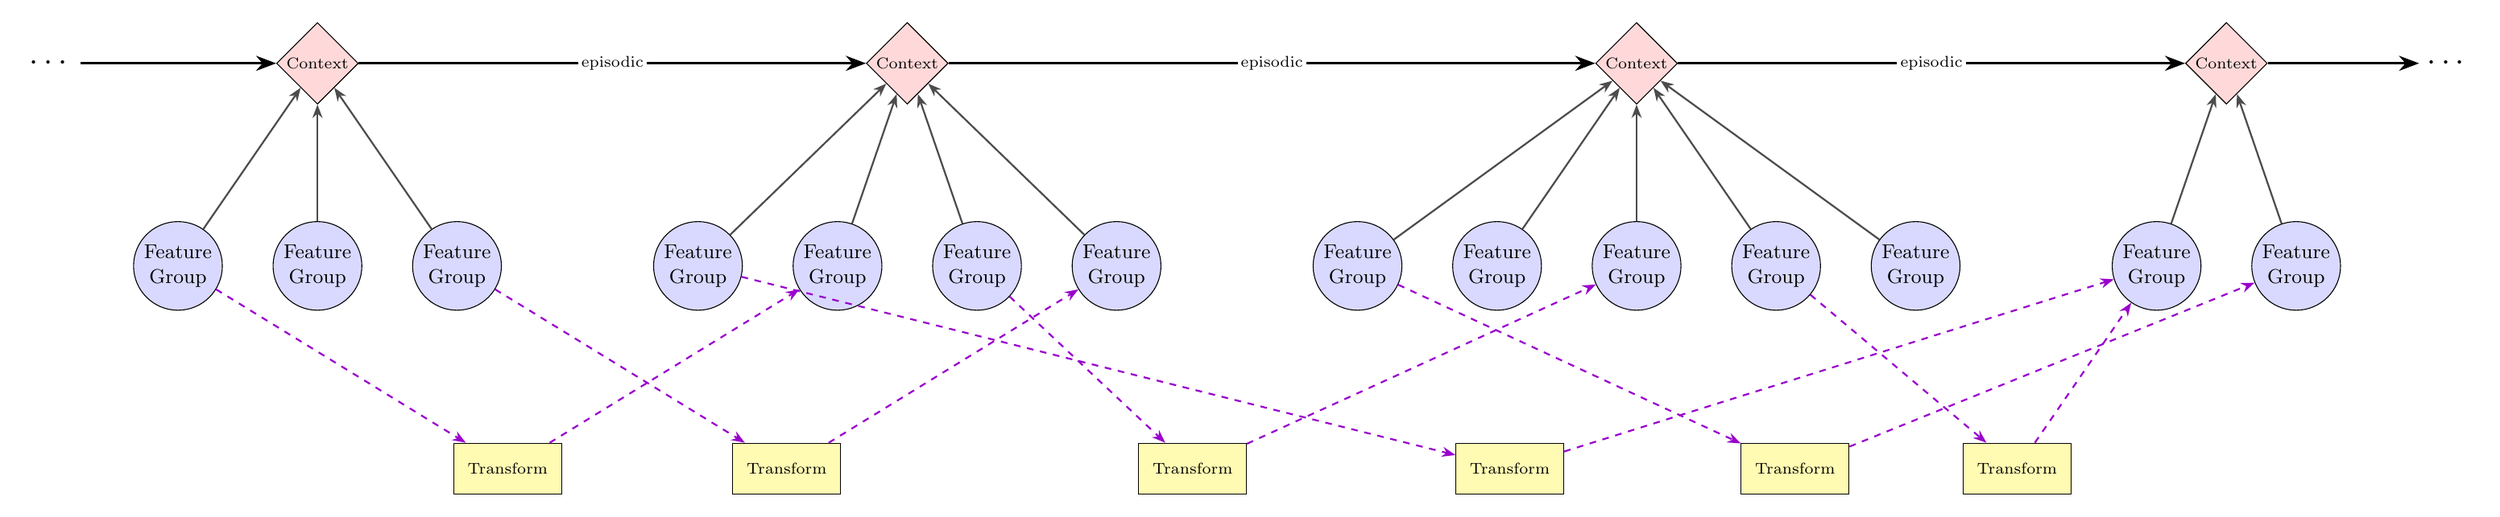
\begin{tikzpicture}[
    circ/.style={circle, draw, fill=featuregroup, minimum size=1.4cm, font=\small, align=center, inner sep=1pt},
    rel/.style={diamond, draw, fill=context, font=\scriptsize, align=center, inner sep=1pt},
    trans/.style={rectangle, draw, fill=transform, font=\scriptsize, align=center, inner sep=3pt, minimum height=0.8cm, minimum width=1.7cm},
    assoc/.style={-{Stealth[length=6pt]}, thick, color=black!70},
    epi/.style={-{Stealth[length=9pt]}, line width=1.1pt, color=black},
    tedge/.style={-{Stealth[length=6pt]}, thick, dashed, color=transformedge},
    lbl/.style={font=\scriptsize, fill=white, inner sep=1.5pt, align=center},
    x=1cm, y=1cm
  ]
    % feature groups (middle row)
    \node[circ] (fg1)  at (0,0)    {Feature\\Group};
    \node[circ] (fg2)  at (2.2,0)  {Feature\\Group};
    \node[circ] (fg3)  at (4.4,0)  {Feature\\Group};
    \node[circ] (fg4)  at (8.2,0)  {Feature\\Group};
    \node[circ] (fg5)  at (10.4,0) {Feature\\Group};
    \node[circ] (fg6)  at (12.6,0) {Feature\\Group};
    \node[circ] (fg7)  at (14.8,0) {Feature\\Group};
    \node[circ] (fg8)  at (18.6,0) {Feature\\Group};
    \node[circ] (fg9)  at (20.8,0) {Feature\\Group};
    \node[circ] (fg10) at (23.0,0) {Feature\\Group};
    \node[circ] (fg11) at (25.2,0) {Feature\\Group};
    \node[circ] (fg12) at (27.4,0) {Feature\\Group};
    \node[circ] (fg13) at (31.2,0) {Feature\\Group};
    \node[circ] (fg14) at (33.4,0) {Feature\\Group};

    % contexts (top row) on the episodic timeline
    \node[rel] (rg1) at (2.2,3.2)  {Context};
    \node[rel] (rg2) at (11.5,3.2) {Context};
    \node[rel] (rg3) at (23.0,3.2) {Context};
    \node[rel] (rg4) at (32.3,3.2) {Context};
    \node[font=\Large] (eb) at (-2.0,3.2) {$\cdots$};
    \node[font=\Large] (ea) at (35.8,3.2) {$\cdots$};


    % transforms (bottom row)
    \node[trans] (t1) at (5.2,-3.2)  {Transform};
    \node[trans] (t2) at (9.6,-3.2)  {Transform};
    \node[trans] (t3) at (16.0,-3.2) {Transform};
    \node[trans] (t4) at (21.0,-3.2) {Transform};
    \node[trans] (t5) at (25.5,-3.2) {Transform};
    \node[trans] (t6) at (29.0,-3.2) {Transform};

    % episodic timeline (thick before/after links)
    \draw[epi] (eb)  -- (rg1);
    \draw[epi] (rg1) -- (rg2) node[lbl, pos=0.5] {episodic};
    \draw[epi] (rg2) -- (rg3) node[lbl, pos=0.5] {episodic};
    \draw[epi] (rg3) -- (rg4) node[lbl, pos=0.5] {episodic};
    \draw[epi] (rg4) -- (ea);

    % relation edges: each Feature Group relates into its Context.
    % Abbreviated -- these stand for the ContextRelationship nodes that the
    % Context aggregates, drawn in full in fig:context. Labels removed; the
    % caption carries the statement.
    \draw[assoc] (fg1)  -- (rg1);
    \draw[assoc] (fg2)  -- (rg1);
    \draw[assoc] (fg3)  -- (rg1);
    \draw[assoc] (fg4)  -- (rg2);
    \draw[assoc] (fg5)  -- (rg2);
    \draw[assoc] (fg6)  -- (rg2);
    \draw[assoc] (fg7)  -- (rg2);
    \draw[assoc] (fg8)  -- (rg3);
    \draw[assoc] (fg9)  -- (rg3);
    \draw[assoc] (fg10) -- (rg3);
    \draw[assoc] (fg11) -- (rg3);
    \draw[assoc] (fg12) -- (rg3);
    \draw[assoc] (fg13) -- (rg4);
    \draw[assoc] (fg14) -- (rg4);

    % transform edges: earlier Feature Group -> Transform -> later Feature Group
    \draw[tedge] (fg1)  -- (t1);  \draw[tedge] (t1) -- (fg5);
    \draw[tedge] (fg3)  -- (t2);  \draw[tedge] (t2) -- (fg7);
    \draw[tedge] (fg6)  -- (t3);  \draw[tedge] (t3) -- (fg10);
    \draw[tedge] (fg4)  -- (t4);  \draw[tedge] (t4) -- (fg13);
    \draw[tedge] (fg8)  -- (t5);  \draw[tedge] (t5) -- (fg14);
    \draw[tedge] (fg11) -- (t6);  \draw[tedge] (t6) -- (fg13);
  \end{tikzpicture}%
  }
  \caption{The Episodic Timeline links successive Contexts -- the point-in-time snapshots of Figure~\ref{fig:context} -- with before/after \emph{episodic} edges, forming an ongoing record of the environment. Each Context relates the Feature Groups present at that point in time, and each \emph{Transform} captures how a Feature Group changes between one point in time and a later one. The edges running from each Feature Group up to its Context are drawn in abbreviated form: a Feature Group has no edge to a Context, but rather edges to the \emph{ContextRelationship} nodes -- one for every pair of Feature Groups, for every relation type -- which the Context in turn aggregates, as Figure~\ref{fig:context} draws in full. Those nodes are omitted here for legibility. (The ``before'' and ``after'' ellipses indicate that the timeline extends indefinitely in both directions.)}
  \label{fig:episodic-timeline}
\end{figure}

\subsection{Probabilistic Edges}
There are two types of probabilistic edges: a PresenceEdge that is used to indicate that the relationship is or isn't present and a ValueEdge that is used to represent both presence and the the probability distribution of a perceptual feature (e.g. the probability distribution of a certain hue or brightness for a color).

The types of relationships that are sculpted are:
\begin{itemize}
    \item Concept $\dashrightarrow$ FeatureGroup / ConceptInstance
    \item FeatureGroup $\rightsquigarrow$ Feature
    \item (Concept, Context) $\dashrightarrow$ Transform
    \item Concept $\rightsquigarrow$ ContextRelationship
    \item ContextRelationship $\dashrightarrow$ Context
    \item source FeatureGroup $\rightsquigarrow$ Transform $\rightsquigarrow$ destination FeatureGroup
    \item Context $\rightsquigarrow$ Significance
    \item source Context $\rightsquigarrow$ Action $\rightsquigarrow$ destination Context
\end{itemize}

Where $\dashrightarrow$ is a PresenceEdge and $\rightsquigarrow$ is a ValueEdge. 

PresenceEdges carry a Beta count of how often the target of the edge was present versus absent when the structure was matched. When an expected edge is present $a$ updates $a' = a+1$, and when an expected edge is absent $b$ is updated $b' = b+1$. The presence probability $a/(a+b)$ is the edge's \emph{criteriality}: how necessary the target is during the matching process. It also provides occlusion and variation robustness: an expected-but-absent relationship is not disqualifying, it contributes $1 - a/(a+b)$ to the match. This aids in feature recognition, where a feature may be occluded; and it aids in concept-context relationships where a missing concept will still yield a context that may still have relevant predictions.

ValueEdges extend the functionality of PresenceEdges. In addition to the Beta values on a PresenceEdge, ValueEdges carry a Normal-Gamma conjugate prior that is "sculpted" during the use of the edge to determine the probability of the nodes along the edge being a match. The Normal-Gamma summary takes the form $(\mu, \kappa, \alpha, \beta)$.

\begin{itemize}
    \item $\mathbf{\mu}$, the current best estimate of the feature's value for this concept (the Normal-Gamma mean);
    \item $\mathbf{\kappa}$, the *effective evidence* behind $\mu$ — its "virtual sample size" — which also sets how much a new observation moves the estimate and how strongly the edge resists being overturned
    \item $\mathbf{\alpha}$, the Gamma shape, accumulating evidence about the feature's precision;
    \item $\mathbf{\beta}$, the Gamma rate, accumulating observed squared deviation, so that $\alpha_{NG}/\beta$ estimates the precision (tightness) of the feature for this concept.
\end{itemize}

\subsection{Concept Matching \& Acquisition}\label{sec:matching}
Matching is a synonym for recognition and recall --- after receiving the FeatureGroup from saliency and cross-modal attention mechanisms, matching reads the ontology graph and to find the best fitting Concept and / or Context. In order to create and maintain a structure that accurately represents the world, any FeatureGroup that is not matched is Acquired as a new Concept, which makes Matching and Acquisition two halves of the same process. Where a match is found between a FeatureGroup and an existing Concept, it is routed to Sculpting mechanisms (see Section \ref{sec:sculpting}) to further refine the edges of the Concept or Context for future use. The matching process that leads to either Acquisition or Sculpting is a single comparison using the mechanism described below.

\paragraph{Candidate Concepts}
The Features in the incoming FeatureGroup act as an inverse index to create a set of candidate Concepts to be evaluated as a potential match for the FeatureGroup -- each Feature in the incoming FeatureGroup also has edges that link to the FeatureGroups associated with Concepts. While this may seem like a large set, the calculation is highly parallelize-able and optimizations can be taken to terminate early based on whether concepts being evaluated can reasonably beat candidates at the top of the list. \hl{TODO: how would this calculation work}. As an additional optimization, there is also a fast-path for assembling a candidate group of Concepts. The fast path is top-down, using the currently active Context to prime the Concepts that it expects to be present.

\paragraph{Existing Concepts versus New Concepts}
The intuitive way to score each candidate Concept would be to create a distance function that compares each candidate Concept to the incoming FeatureGroup and the candidate with the lowest distance (e.g. most features and values in common between the candidate Concept and the target FeatureGroup) would win that match; however, this leads to wrong matches in cold-start scenarios where few Concepts are available and even Concepts with very little overlap with the FeatueGroup would incorrectly be the best match. This might be solved by having a minimum threshold required for how many Features must match between a candidate Concept and the target FeatureGroup; however, that threshold would end up being world and Context specific and ultimately be the source of high error rates \hl{TODO: we need to make this argument more compelling}. That threshold can be avoided if instead a hypothesis of "this is a Concept that doesn't yet exist in the ontology" is created and competes with candidate Concepts. That novelty hypothesis must have two things: 1) an account of what it expects to observe, so that it can be scored on evidence like any candidate Concept; and 2) a prior probability that it applies at all.

To the first point of what a novelty hypothesis expects to observe -- it expects nothing out of the ordinary. That is, it expects each feature type to be present at the same rate that they appear in the world, and the values of the feature can be any value. To be more precise, there are two background quantities: the quantity of feature types, $q_f$, is the background presence rate of feature type $f$: the fraction of bound FeatureGroups in which $f$ appears at all. It is a Beta counter carried on the Feature node itself, updated every time a FeatureGroup is created. It is created with the value $\mathrm{Beta}(1,1)$, so an agent with no experience begins at $q_f = 1/2$ --- \hl{TODO: is this right?} a coin flip as to whether the feature is present at or not. The second background quantity for a new Concept, $g_{0,f}$, is the base density over values: uniform across the extractor's calibrated output range, $g_{0,f}(x) = 1/(\mathrm{hi}_f - \mathrm{lo}_f)$, the maximum-entropy density on a bounded interval and \hl{TODO} hence the flat value prior a newly acquired structure has before any observation constrains it. Unlike $q_f$, $g_{0,f}$ is never updated and is just the static calibrated output range for each feature extractor.

The second point is that a novelty hypothesis needs a prior probability for determining whether a new concept should be created. For this we use the Good--Turing \cite{good_population_1953} approach, which uses the number of singular observations, $N_1$, as the prior for finding a never before observed observation. The this gives us the standard form for the probability of a new Concept as:

$$p_{\mathrm{new}} \;=\; \frac{N_1 + 1}{n + 2}$$

where $N_1$ is the decayed total of FeatureGroups that have only been observed once, and $n$ is the decayed total of attendance events. The equation includes Laplace smoothing to keep the values between 0 and 1 at the extreme cases of no observations and all observations are unique to prevent locking on no new Concepts or all new concepts, respectively. Note that one encounter is counted as the total the life of a FeatureGroup as it is tracked across ticks; otherwise, each FeatureGroup would be counted as a second occurrence on the second tick and it would be removed from $N_1$, meaning that there would never be any unique observations beyond a single tick. This approach also puts pressure on the accuracy of tracking -- if tracking loses and re-acquires a novel concept, it now counts as "twice" and gets dropped from Good--Turing's $N_1$. Both $N_1$ and $n$ are subject to a decay factor, $\rho$, which defines the sliding recency window for the frequency of new concepts. The decay factor is:

$\tilde{n}_{\max} = 1/(1-\rho)$

$$\tilde{a}_C \longleftarrow \rho\,\tilde{a}_C + \mathbf{1}[C \text{ attended}]\, \qquad \tilde{a}_C \geq 1$$

\hl{TODO: decay}

\paragraph{Concept Scoring}
Based on the specification of novelty hypothesis's in the previous section, it can now compete directly with the candidate Concepts. Because novelty hypothesis describes an unremarkable observation, it is also the natural reference against which remarkable ones are measured. So rather than asking how probable an observation is under a candidate --- a quantity with no interpretable scale --- we ask how much \emph{better} the candidate explains it than the background does. Each feature type contributes one additive term, in log units, to the score of a candidate FeatureGroup $F$, and evidence accumulates by summation:

$$
s_f(F) \;=\;
\begin{cases}
\log\dfrac{a/(a+b)}{q_f} \;+\; \log\dfrac{\mathrm{St}\!\left(x_f \mid \mu,\kappa,\alpha,\beta\right)}{g_{0,f}(x_f)} & \text{$f$ expected and present with value $x_f$,}\\[10pt]
\log\dfrac{1 - a/(a+b)}{1 - q_f} & \text{$f$ expected and absent,}\\[10pt]
0 & \text{no edge for $f$,}
\end{cases}
$$

In the first case, we separate \emph{confirmation} from \emph{information}: a feature contributes more to a Concept's candidate score based on: the more strongly the Concept $C$ expects the feature than the background rate of the feature in the world (criteriality $a/(a+b)$ against the background rate $q_f$). Dividing the edge's Student-$t$ predictive by the flat base density means a candidate earns nothing merely for being precise, only for being precise \emph{and right}, while a vague prediction correctly earns near zero whether it is confirmed or not. The better that the observed value fits the edge's Student-$t$ predictive $\mathrm{St}(\cdot \mid \mu,\kappa,\alpha,\beta)$ than a value drawn from anywhere in the extractor's range.

In the second case, $C$ is charged for expecting a feature that is not present, priced against how surprising that absence would be by chance. Because the presence counts in an edge are initialized with $\mathrm{Beta}(1,1)$ the charge is always finite and features missing due to occlusion only degrade a match but never disqualify it.

Note that the $q_f$ denominators also make rare features weigh more than common ones: a feature that is rare in the world but expected by the concept is stronger evidence for $C$ than a more common feature.

Finally, in the third case, the feature is contribution is identical for both the Concept and the novelty hypothesis, causing $q_f$ and $g_{0,f}$ to cancel out.

Deciding whether a candidate Concept is a match to the present features is performed by comparing the candidate versus a reserved novelty hypothesis $\nu$ -- a reserved share of probability mass representing a new Concept that is not yet represented in the ontology. $\nu$ is always calculated in parallel with the candidate Concept on the same evidence, with the expectation that features are present at exactly their background rate, accepting any value in the range of the feature, and paying the same charge for expected but missing features.

$$
C^{*} \;=\; \operatorname*{arg\,max}_{C \,\in\, \mathcal{C} \,\cup\, \{\nu\}} \Big[\, \log \pi_C \;+\; \sum_{f} s_f(C) \,\Big],
\qquad \pi_\nu = p_{\mathrm{new}},
$$

where $\mathcal{C}$ is the candidate set and $\pi_C$ is a candidate's prior weight the prior weights are normalized so that $\sum_C \pi_C = 1 - p_{\mathrm{new}}$. A match is declared exactly when some existing Concept outscores $\nu$ and a new Concept is acquired exactly when $\nu$ outscores every existing candidate.

Note that while a single Concept (new or existing) wins the match, the runner-ups are not discarded. They are used by the Prediction Monitors (Section \ref{sec:prediction}) as fall-backs for if prediction fails and as candidates for Abstraction (Section \ref{sec:abstraction}).

\paragraph{Acquisition}
A concept is acquired when the novelty hypothesis wins the matching competition. That is, no existing structure in the ontology offered a better explanation of the features that were observed than creating a new concept.

The edges of the new Concept are formed by applying one iteration of the standard Sculpting update (Section \ref{sec:sculpting}) to the features that were observed to create the new Concept. For a founding feature observed with value $x$,

$$
(a, b) = (2, 1), \qquad (\mu, \kappa, \alpha, \beta) = \left(x,\; 1,\; 1,\; \sigma_f^2\right),
$$

where the presence counts are the innate $\mathrm{Beta}(1,1)$ plus the founding sighting (criteriality $2/3$) and $\sigma_f$ is the extractor's noise floor. This one-shot acquisition primes the concept so that is able to be recalled for future matching and prediction, albeit weakly until it is sculpted and reinforced over time.

The reserved mass $p_{\mathrm{new}}$ is not a constant; it is estimated from the agent's own recent rate of genuine first encounters, in the manner of Good--Turing missing-mass estimation \hl{citation: Good 1953}.

- \hl{TODO} Concepts are the locus of predictability and transferability. They have relationships to all their (retained) concept instances, the relationships that were present in those instances, and the transforms that occurred in those instances. This enables them to identify similar circumstances based on the other concepts present and apply the same transforms under those conditions to predict or simulate what will happen in future situations.

It should be noted that matching and acquisition do not need to be perfect. If the wrong Concept or Context is selected by matching, downstream Prediction Monitors (Section \ref{sec:prediction}) will identify that the Concept and Context are not correctly forecasting accurately and trigger a process to re-identify concepts. Likewise, for acquisition -- if the wrong Concepts or Contexts are acquired, they will be abstracted to their correct counterparts or their edges will eventually be Sculpted to the point where they are unreachable and forgotten.

\subsection{Context Matching \& Acquisition}
- Uses a similar process to Concept Matching \& Acquisition
- Matches based on FeatureGroups and Relationships. Note that all Concepts AND their Relationships must exactly match, which is critical for Prediction
- New Contexts are acquired when no exactly matching Context exists

\subsection{Sculpting Edges}\label{sec:sculpting}
When a concept is successfully matched, the edges that that are used for the match have their probabilities increased information and the edges that were expected but absenthave their probabilities decreased (i.e. the edges are "sculpted"). Note that inheritance relationships are not sculpted and thus aren't described in this section. See Section \ref{sec:abstraction} for more about inheritance.

On the n-th consistent observation x, the standard Normal-Gamma updates are

$$\mu' = \frac{\kappa\mu + x}{\kappa + 1}, \qquad \kappa' = \kappa + 1, \qquad \alpha' = \alpha + \tfrac{1}{2}, \qquad \beta' = \beta + \frac{\kappa}{\kappa+1}\cdot\frac{(x - \mu)^2}{2}.$$

See Section \ref{pseudocode:edges} for pseudocode detailing the implementation of Edges.

\begin{figure}[ht]
  \centering
  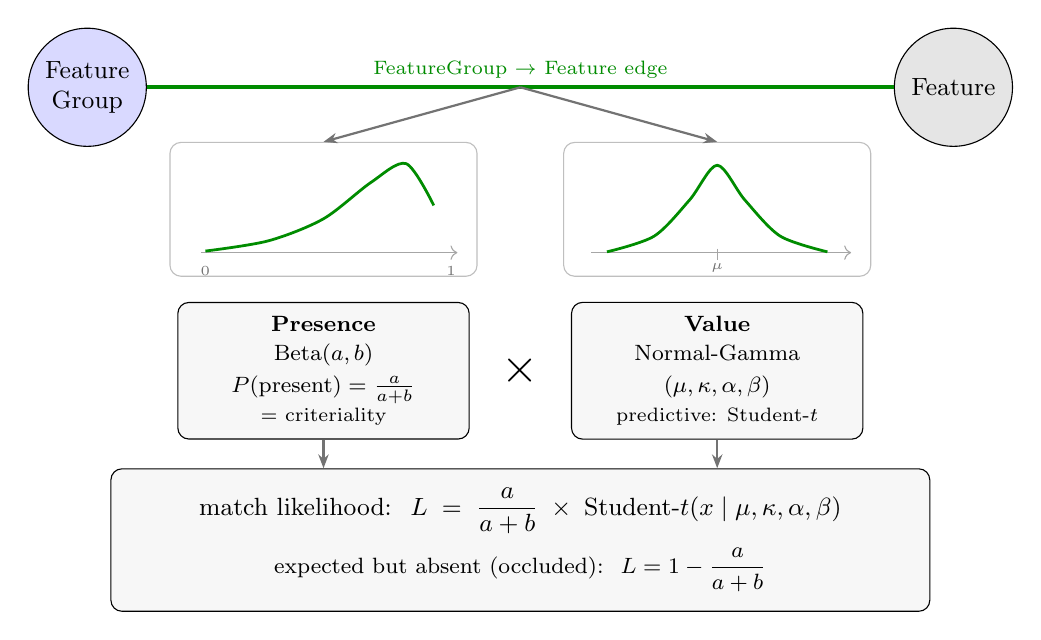
\begin{tikzpicture}[
    fgrp/.style={circle, draw, fill=featuregroup, minimum size=1.5cm, font=\small, align=center, inner sep=1pt},
    feat/.style={circle, draw, fill=feature, minimum size=1.5cm, font=\small, align=center, inner sep=1pt},
    chip/.style={rectangle, draw, rounded corners, fill=black!3, align=center, inner sep=5pt, minimum width=3.7cm, font=\footnotesize},
    icon/.style={rectangle, draw=black!25, rounded corners, fill=white, minimum width=3.9cm, minimum height=1.7cm},
    cedge/.style={line width=1.4pt, color=conceptedge},
    pin/.style={-{Stealth[length=5pt]}, thick, color=black!55},
    edgelbl/.style={font=\scriptsize, fill=white, inner sep=1.5pt},
    x=1cm, y=1cm
  ]
    % --- the two real nodes and the single edge between them ---
    \node[fgrp] (c) at (0,0)  {Feature\\Group};
    \node[feat] (f) at (11,0) {Feature};
    \draw[cedge] (c) -- (f) node[edgelbl, midway, above=1pt] {FeatureGroup $\to$ Feature edge};
    \coordinate (mid) at (5.5,0);

    % --- distribution icons (top of each column) ---
    % presence icon: skewed Beta, mass near 1 (a criterial, usually-present feature)
    \node[icon] (pi) at (3.0,-1.55) {};
    \begin{scope}[shift={(3.0,-1.55)}]
      \draw[->, black!35] (-1.55,-0.55) -- (1.7,-0.55);
      \draw[line width=1pt, conceptedge] plot[smooth] coordinates
        {(-1.5,-0.53) (-0.7,-0.4) (0,-0.12) (0.6,0.34) (1.05,0.58) (1.4,0.05)};
      \node[font=\tiny, black!55] at (-1.5,-0.78) {0};
      \node[font=\tiny, black!55] at (1.62,-0.78) {1};
    \end{scope}
    % value icon: Gaussian bell centered on mu
    \node[icon] (vi) at (8.0,-1.55) {};
    \begin{scope}[shift={(8.0,-1.55)}]
      \draw[->, black!35] (-1.6,-0.55) -- (1.7,-0.55);
      \draw[line width=1pt, conceptedge] plot[smooth] coordinates
        {(-1.4,-0.54) (-0.8,-0.34) (-0.35,0.12) (0,0.56) (0.35,0.12) (0.8,-0.34) (1.4,-0.54)};
      \draw[black!35] (0,-0.5) -- (0,-0.64) node[font=\tiny, black!55, below, inner sep=1pt] {$\mu$};
    \end{scope}

    % --- pins from the edge down to each icon ---
    \draw[pin] (mid) -- (pi.north);
    \draw[pin] (mid) -- (vi.north);

    % --- text chips (below each icon) ---
    \node[chip] (pc) at (3.0,-3.6) {\textbf{Presence}\\[1pt] $\mathrm{Beta}(a,b)$\\[2pt] $P(\mathrm{present})=\frac{a}{a+b}$\\[1pt] {\scriptsize $=$ criteriality}};
    \node[chip] (vc) at (8.0,-3.6) {\textbf{Value}\\[1pt] Normal-Gamma\\[2pt] $(\mu,\kappa,\alpha,\beta)$\\[1pt] {\scriptsize predictive: Student-$t$}};

    % --- multiply symbol between the two chips ---
    \node[font=\LARGE] at (5.5,-3.6) {$\times$};

    % --- combined likelihood (bottom) ---
    \node[rectangle, draw, rounded corners, fill=black!3, align=center, inner sep=7pt, minimum width=10.4cm, font=\small]
      (comb) at (5.5,-5.75)
      {match likelihood:\; $L \;=\; \dfrac{a}{a+b}\;\times\;\text{Student-}t\!\left(x \mid \mu,\kappa,\alpha,\beta\right)$\\[4pt]
       {\footnotesize expected but absent (occluded):\; $L = 1 - \dfrac{a}{a+b}$}};
    \draw[pin] (pc.south) -- (comb.north -| pc.south);
    \draw[pin] (vc.south) -- (comb.north -| vc.south);
  \end{tikzpicture}
  \caption{Anatomy of a ValueEdge: the edge from a Feature Group to one of its Features, which is the unit the matching score sums over. Every ValueEdge stores two conjugate summaries, sculpted independently: a \emph{presence} distribution (Beta counts, whose mean $a/(a+b)$ is the feature's \emph{criteriality}) and a \emph{value} distribution (Normal-Gamma). Matching multiplies the two into a single match likelihood; an expected-but-absent feature contributes $1-a/(a+b)$ rather than disqualifying the match. Features attach to Feature Groups, never to Concepts; a Concept reaches its Features only through the Feature Groups it holds.}
  \label{fig:edge-anatomy}
\end{figure}

\paragraph{Retention / Forgetting}
- Repetition through recall leads to retention (i.e. reinforcement). Every successful recall sculpts edges to increase their probability of their associated concepts being referenced in the future.
- Forgetting is the process of reducing the weight of edges through decay (i.e. the effective evidence $\kappa$ and the presence counts decay towards a plasticity floor). Edges are not removed, but lose their priority in recall and / or reduce their confidence. "Forgotten" concepts are hard to reach but not gone and on re-encounter they can be recalled and the edges will quickly increase in confidence to restore its utility.
- Forgetting is essential to the plasticity of the agent -- de-prioritizing old information allows new information to be utilized in the correct context. For example, if an object is moved the agent must be able to reduce the probability of the old location and increase the probability of the new location so that it can be recalled in the correct context.
- Explains both aspects of forgetting due to interference: retroactive interference occurs because the graph develops new, stronger relationships that make old relationships difficult to reach; proactive interference because the weights are already established heavily in favor of historical concepts.

\citep{ryan_frankland_2022, underwood_1957, oleary_natural_2024, bjork_bjork_1992}

\subsection{Prediction}\label{sec:prediction}
Prediction uses the current Context, Concepts, FeatureGroups, and their associated Transforms to predict the immediate next tick of the agent, and whether the prediction was accurate or not is used as a trigger for confidence building or error correction. Prediction starts with matching similar Concepts and Contexts. Prediction has three parts: 1) predicting the next tick; 2) resolving whether the prediction from the previous tick was accurate or not; 3) monitoring predictions over multiple ticks and multiple concepts for potential error correction and abstraction.

\paragraph{Predicting the next tick}
In the typical scenario, an agent will have an identified Context that can use its relationships to identify Transforms to apply to predict the next tick. Note that the Episodic Timeline graph of Section \ref{sec:episodic-timeline} can be refactored to be Concept-centric (see \ref{fig:concept-structure}):

\begin{figure}[ht]
  \centering
  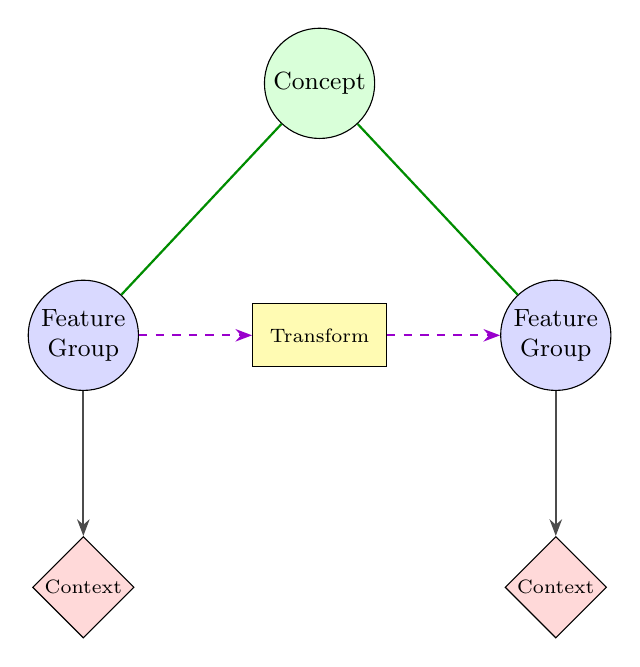
\begin{tikzpicture}[
    conc/.style={circle, draw, fill=concept, minimum size=1.4cm, font=\small, align=center, inner sep=1pt},
    circ/.style={circle, draw, fill=featuregroup, minimum size=1.4cm, font=\small, align=center, inner sep=1pt},
    rel/.style={diamond, draw, fill=context, font=\scriptsize, align=center, inner sep=1pt},
    trans/.style={rectangle, draw, fill=transform, font=\scriptsize, align=center, inner sep=3pt, minimum height=0.8cm, minimum width=1.7cm},
    cedge/.style={thick, color=conceptedge},
    tedge/.style={-{Stealth[length=6pt]}, thick, dashed, color=transformedge},
    assoc/.style={-{Stealth[length=6pt]}, thick, color=black!70},
    x=1cm, y=1cm
  ]
    \node[conc]  (cpt) at (0,3.2)   {Concept};
    \node[circ]  (fg1) at (-3,0)    {Feature\\Group};
    \node[circ]  (fg2) at (3,0)     {Feature\\Group};
    \node[trans] (t)   at (0,0)     {Transform};
    \node[rel]   (rg1) at (-3,-3.2) {Context};
    \node[rel]   (rg2) at (3,-3.2)  {Context};

    % concept linked to its two feature groups (green lines)
    \draw[cedge] (cpt) -- (fg1);
    \draw[cedge] (cpt) -- (fg2);
    % transform between the two feature groups
    \draw[tedge] (fg1) -- (t);
    \draw[tedge] (t) -- (fg2);
    % each feature group relates into its context
    \draw[assoc] (fg1) -- (rg1);
    \draw[assoc] (fg2) -- (rg2);
  \end{tikzpicture}
  \caption{A Concept (green) retains links to the Feature Groups that instantiate it. Two such Feature Groups are shown, together with the \emph{Transform} that captures the change between them and the \emph{Context} that each one participated in.}
  \label{fig:concept-structure}
\end{figure}

Each (Context, FeatureGroup) pair has a Transform associated with it, as discussed previously in the Episodic Timeline section. Prediction then is simply applying the previously captured transforms to each Concept in the Context to predict where each Concept will be in the next state. Across all the potential transforms for a single Concept the Transforms to apply are calculated using:

$$
T^{*} \;=\; \operatorname*{arg\,max}_{T \,\in\, \mathcal{T}(C, K)} \; \frac{a_T}{a_T + b_T},
$$

where $\mathcal{T}(C, K)$ is the set of transforms recorded for Concept $C$ in Context $K$ and $(a_T, b_T)$ are the transform edge's Beta counts. $T^{*}$'s deltas are applied as point values to produce the predicted next state. Note that transforms are calculated and applied at the FeatureGroup, ensuring that Concepts with different relationships within the Context will predict according to their specific situations. For example, the Concept of a marble may have a position Transform associated with it if it is expected to roll. If there are two marbles present and one is on a flat, level surface and the other on an incline, the one on the flat surface would not apply the motion Transform (due to its relationship to the flat surface) and the one on the incline would apply the motion Transform (due to its relationship with the incline surface) -- the same Concept with two different instances, where each instance predicts separately.

There are scenarios where Concepts may be known from previous experience; however, they are combined in a novel Context (e.g. experiencing a familiar object in a new place). In this scenario, the most similar previous Context associated with the Concept are used for prediction, enabling transfer of the Concept from an old Context to a new Context.

If a Concept is newly Acquired and has no Transforms associated with it, there is no prediction that can be made -- only observation to acquire new Transforms for future use.

\hl{TODO?} Finally, as time moves forward and motion and change comes into play, the Transformations between FeatureGroups associated with a concept can remove any final ambiguity if there are multiple potentially matching concepts or if the overall similarity based on Features and Contexts alone was low.

\paragraph{Resolving predictions}
At the start of each tick, the prediction from the previous tick is evaluated to determine if the prediction was accurate. FeatureGroups are tracked across frames by low-level mechanisms. For each feature that was in the original FeatureGroup the features are compared to the new FeatureGroup. Only features that exist in both groups are compared, otherwise the features are ignored to account for occlusion. 

\paragraph{Prediction monitoring}
Each Concept instance in a scene has an associated Prediction Monitor that aggregates a record of how well the transforms for the Concept predicted the next state. The monitor is used to decide whether the wrong Concept is being applied \hl{TODO and...}. The Prediction Monitor's state is a running to total $W$ (in log units) of how much better rival explanations have predicted the instance's outcomes than the held Concept has. The monitor fires when:

$$
W \;\geq\; \log \frac{1}{\alpha_r(v)},
$$

where $\alpha_r$ is the lifetime probability that the monitor ever fires while the matched Concept remains an adequate predictor of the instance and the current valence magnitude $v$ lowers the boundary. \hl{TODO}

\subsection{Concept Abstraction, Hoisting, Inheritance}\label{sec:abstraction}
- Abstraction is how hierarchies of Concepts and Contexts are created
- Abstraction is the mechanism that provides transference of knowledge: concepts in the same families are expected to provide the same predictions via their Transforms
- Predicting the same is what makes Concepts candidates for abstraction. Matching identifies not only the current Concept that is the best match for a FeatureGroup, but also runner-up Concepts that beat the novelty hypothesis but were not the winners of the competition. The winner and the runner-ups are tracked by prediction monitors, and if they predict the same transforms (right or wrong), they are candidates for abstraction.
- Abstraction is an economic savings for three reasons: 1) rather than holding on to a large amount of detail, only the necessary detail for the high-confidence predictions needs to be retained; 2) relationships can be formed and predictions can happen at higher levels, enabling faster predictions; 3) the newly extracted / abstracted concepts can be applied to more scenarios and newly encountered scenarios, enabling transference of knowledge / prediction.
- Abstraction is a different mechanism than reification. Reification uses strength of sculpted edges as a grouping mechanism, not co-activation and co-prediction.
- When a new level of concept is created, it hoists up the common contexts, relationships, feature groups, and transforms -- adding them to the new parent concept and removing them from the common concepts.
- Child concepts inherit the contexts, feature groups, and transforms of their parents -- the common "dog" class of features and behaviors applies to all its children. Individual children can override the inheritance by retaining or adding specific features, contexts, or transforms to their own concepts enabling child-concept specific predictions. For example, "all dogs are generally nice but Fido tries to bite".
- Transforms can be abstracted to concepts. This enables reasoning and transference around concepts such as "fast" and "to the left"
- The concept instances that contribute to the concept also contribute their known relationships and previous behaviors: the concept is expected to behave the same when the concepts surrounding it are the same.
- This process is iterative: concepts can be iteratively abstracted, not requiring grounded concepts to form higher-level concepts. (See iterative / recursive abstraction below)
- The same mechansims are used for Contexts to create a hierarchy of Contexts

\citep{mandler_perceptual_2000}

Concept First Layer Abstraction Diagram: \hl{TODO}
Concept Second Layer Abstraction Diagram: \hl{TODO}

\begin{figure}[ht]
  \centering
  \resizebox{\linewidth}{!}{%
  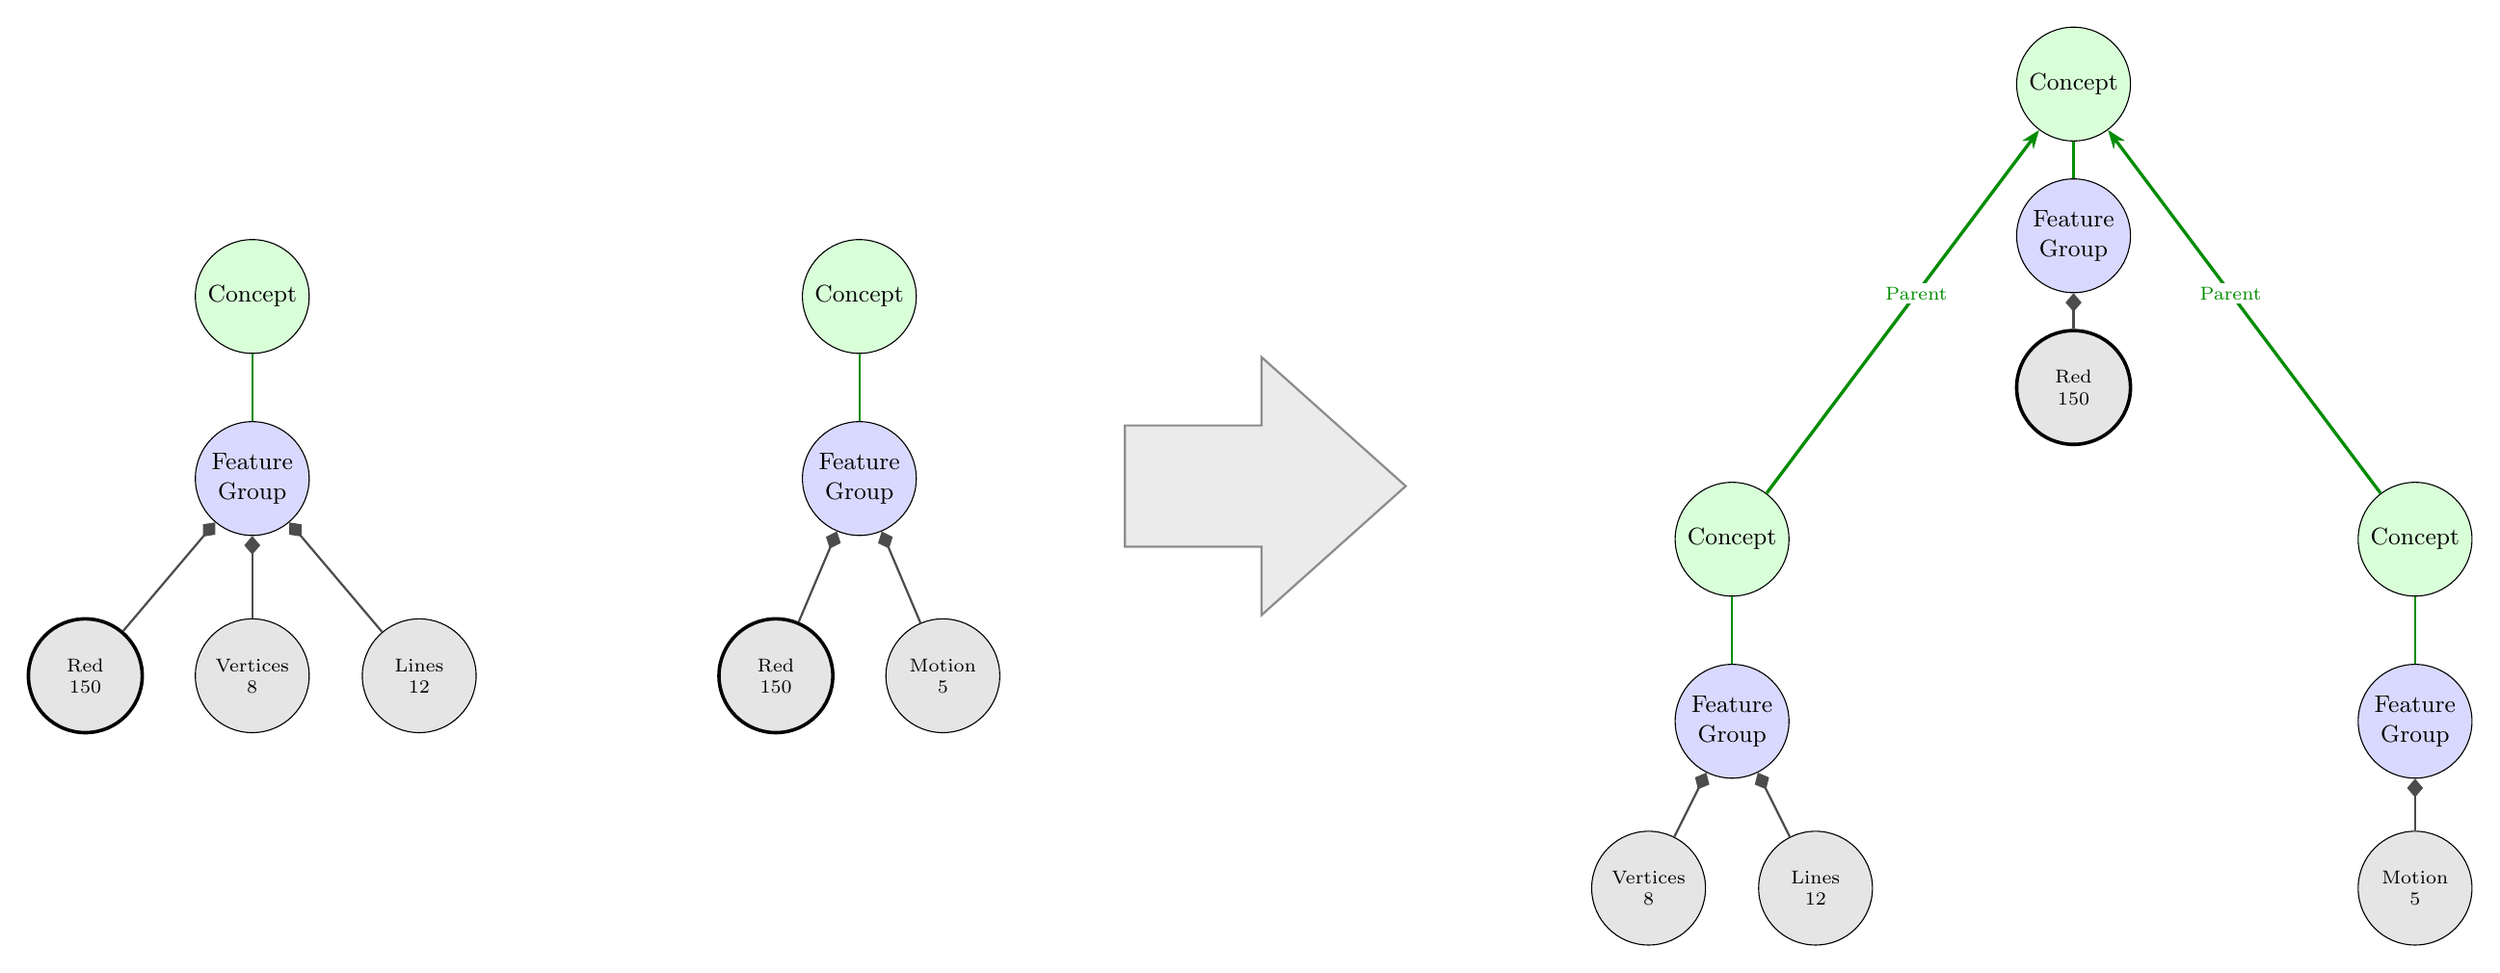
\begin{tikzpicture}[
    conc/.style={circle, draw, fill=concept, minimum size=1.5cm, font=\small, align=center, inner sep=1pt},
    fgrp/.style={circle, draw, fill=featuregroup, minimum size=1.5cm, font=\small, align=center, inner sep=1pt},
    feat/.style={circle, draw, fill=feature, minimum size=1.5cm, font=\scriptsize, align=center, inner sep=1pt},
    shared/.style={feat, line width=1.3pt},
    cedge/.style={thick, color=conceptedge},
    pedge/.style={-{Stealth[length=7pt]}, line width=1.2pt, color=conceptedge},
    agg/.style={{Diamond[length=7pt, width=6pt]}-, thick, color=black!70},
    lbl/.style={font=\scriptsize, fill=white, inner sep=1.5pt, align=center},
    x=1cm, y=1cm
  ]
    % ================= cluster 1 (left) =================
    \node[conc]   (c1)   at (0,7.2)    {Concept};
    \node[fgrp]   (fg1)  at (0,4.8)    {Feature\\Group};
    \node[shared] (f1a)  at (-2.2,2.2) {Red\\150};
    \node[feat]   (f1b)  at (0,2.2)    {Vertices\\8};
    \node[feat]   (f1c)  at (2.2,2.2)  {Lines\\12};

    \draw[cedge] (c1)  -- (fg1);
    \draw[agg]   (fg1) -- (f1a);
    \draw[agg]   (fg1) -- (f1b);
    \draw[agg]   (fg1) -- (f1c);

    % ================= cluster 2 =================
    \node[conc]   (c2)   at (8,7.2)   {Concept};
    \node[fgrp]   (fg2)  at (8,4.8)   {Feature\\Group};
    \node[shared] (f2a)  at (6.9,2.2) {Red\\150};
    \node[feat]   (f2b)  at (9.1,2.2) {Motion\\5};

    \draw[cedge] (c2)  -- (fg2);
    \draw[agg]   (fg2) -- (f2a);
    \draw[agg]   (fg2) -- (f2b);

    % ================= block arrow (unattached) =================
    \draw[fill=black!8, draw=black!45, line width=0.8pt]
      (11.5,3.9) -- (13.3,3.9) -- (13.3,3.0) -- (15.2,4.7)
                 -- (13.3,6.4) -- (13.3,5.5) -- (11.5,5.5) -- cycle;

    % ================= merged cluster (right) =================
    % parent concept, its feature group, and the hoisted common feature
    \node[conc]   (cp)  at (24,10.0) {Concept};
    \node[fgrp]   (fgp) at (24,8.0)  {Feature\\Group};
    \node[shared] (fp)  at (24,6.0)  {Red\\150};

    \draw[cedge] (cp)  -- (fgp);
    \draw[agg]   (fgp) -- (fp);

    % child cluster 1 (common feature removed)
    \node[conc] (c1m)  at (19.5,4.0)   {Concept};
    \node[fgrp] (fg1m) at (19.5,1.6)   {Feature\\Group};
    \node[feat] (f1bm) at (18.4,-0.6)  {Vertices\\8};
    \node[feat] (f1cm) at (20.6,-0.6)  {Lines\\12};

    \draw[cedge] (c1m)  -- (fg1m);
    \draw[agg]   (fg1m) -- (f1bm);
    \draw[agg]   (fg1m) -- (f1cm);

    % child cluster 2 (common feature removed)
    \node[conc] (c2m)  at (28.5,4.0)  {Concept};
    \node[fgrp] (fg2m) at (28.5,1.6)  {Feature\\Group};
    \node[feat] (f2bm) at (28.5,-0.6) {Motion\\5};

    \draw[cedge] (c2m)  -- (fg2m);
    \draw[agg]   (fg2m) -- (f2bm);

    % parent links from each child concept up to the abstracted concept
    \draw[pedge] (c1m) -- (cp) node[lbl, pos=0.55] {Parent};
    \draw[pedge] (c2m) -- (cp) node[lbl, pos=0.55] {Parent};
  \end{tikzpicture}%
  }
  \caption{Abstraction merges common Concepts that predict the same, hoisting up their common Features to the newly created parent Concept. When matching and prediction algorithms are applied, the hoisted Features are inherited down to the child concepts. Abstraction also applies to Transforms, Relationships, and Contexts; however, only Features are shown here for simplicity.}
  \label{fig:abstraction}
\end{figure}

\paragraph{Iterative / Recursive Abstraction}
- Abstract concepts, relationships, transforms across different types into new concepts.
- Iterative abstraction need not be across common types (concept + concept abstraction; etc.); New concepts may be formed on mixed types (concept + relationship abstraction; etc.)
- Example: \hl{TODO}

Iterative Abstraction Diagram(s): \hl{TODO}

\subsection{Reification}
- As the strength of PresenceEdge relationships between a Concept and its FeatureGroups, Relationships, Contexts, or Transforms approaches near certainty (i.e. probability ~1) with no competing relationships, those relationships are refactored to become their own Concepts -- they are "reified" into their own Concepts.
- additive reification leads to mereology relationships: features that regularly occur on the same concept, in the same relationship, and have the same transforms are part of the same Concept (e.g. fingers are part of hand because they move with the hand, have consistent relationships to the hand, and move when the hand moves so they have the same transforms).
- subtractive reification takes an aspect of a Concept and elevates it to its own Concept. For example, creating the concept "red" from a single Feature edge for red that has been sculpted to near certainty. Or "fast" for a single Transform for a large movement in a single tick. this is the source of non-noun Concepts.

\subsection{Sensory Valence}
- Sensory valence (reward and punishment) signals (hunger, pain, pleasure, etc.) are not binary, but are continuous (degree of hunger, degree of pain, degree of pleasure, etc.). The signal is negative for situations to be avoided.
- Sensory valence signals are nodes that are linked to contexts based on the their continuous value as a weight, enabling them to be retrieved when similar situations are encountered: contexts that were tagged with hunger can be recalled when the agent is facing the same signal, enabling it to identify contexts that may aid in the current situation.
- They may also be immediately available during recall to identify near-term objects or actions to steer towards or away from.
- Sensory valence acts as an amplification signal for concept and context acquisition, ensuring that high valence scenarios are available for recall to guide attraction or avoidance in action selection.
- Valence also acts as a multiplier on the novelty threshold: high-stakes prediction failures spawn new structure sooner than low-stakes ones.

\begin{figure}[ht]
  \centering
  \resizebox{\linewidth}{!}{%
  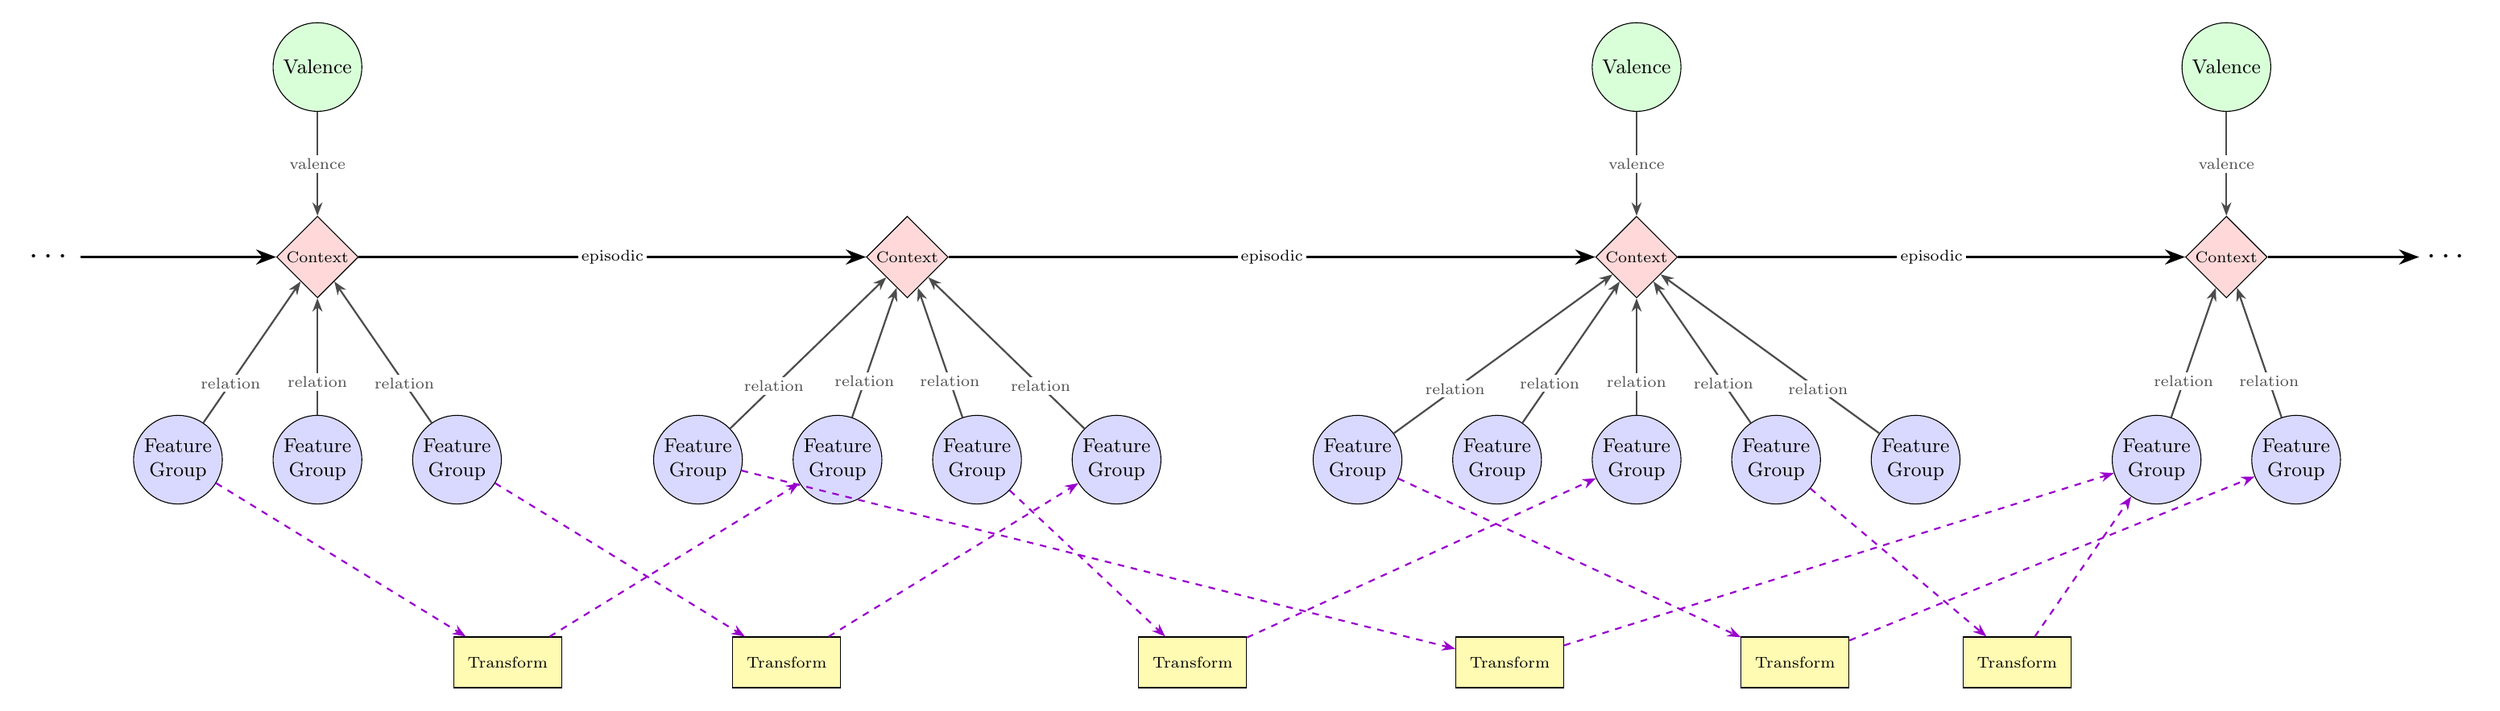
\begin{tikzpicture}[
    circ/.style={circle, draw, fill=featuregroup, minimum size=1.4cm, font=\small, align=center, inner sep=1pt},
    rel/.style={diamond, draw, fill=context, font=\scriptsize, align=center, inner sep=1pt},
    trans/.style={rectangle, draw, fill=transform, font=\scriptsize, align=center, inner sep=3pt, minimum height=0.8cm, minimum width=1.7cm},
    val/.style={circle, draw, fill=green!15, minimum size=1.4cm, font=\small, align=center, inner sep=1pt},
    assoc/.style={-{Stealth[length=6pt]}, thick, color=black!70},
    epi/.style={-{Stealth[length=9pt]}, line width=1.1pt, color=black},
    tedge/.style={-{Stealth[length=6pt]}, thick, dashed, color=transformedge},
    lbl/.style={font=\scriptsize, fill=white, inner sep=1.5pt, align=center},
    x=1cm, y=1cm
  ]
    % feature groups (middle row)
    \node[circ] (fg1)  at (0,0)    {Feature\\Group};
    \node[circ] (fg2)  at (2.2,0)  {Feature\\Group};
    \node[circ] (fg3)  at (4.4,0)  {Feature\\Group};
    \node[circ] (fg4)  at (8.2,0)  {Feature\\Group};
    \node[circ] (fg5)  at (10.4,0) {Feature\\Group};
    \node[circ] (fg6)  at (12.6,0) {Feature\\Group};
    \node[circ] (fg7)  at (14.8,0) {Feature\\Group};
    \node[circ] (fg8)  at (18.6,0) {Feature\\Group};
    \node[circ] (fg9)  at (20.8,0) {Feature\\Group};
    \node[circ] (fg10) at (23.0,0) {Feature\\Group};
    \node[circ] (fg11) at (25.2,0) {Feature\\Group};
    \node[circ] (fg12) at (27.4,0) {Feature\\Group};
    \node[circ] (fg13) at (31.2,0) {Feature\\Group};
    \node[circ] (fg14) at (33.4,0) {Feature\\Group};

    % contexts (top row) on the episodic timeline
    \node[rel] (rg1) at (2.2,3.2)  {Context};
    \node[rel] (rg2) at (11.5,3.2) {Context};
    \node[rel] (rg3) at (23.0,3.2) {Context};
    \node[rel] (rg4) at (32.3,3.2) {Context};
    \node[font=\Large] (eb) at (-2.0,3.2) {$\cdots$};
    \node[font=\Large] (ea) at (35.8,3.2) {$\cdots$};

    % valence tags (above the contexts)
    \node[val] (v1) at (2.2,6.2)  {Valence};
    \node[val] (v2) at (23.0,6.2) {Valence};
    \node[val] (v3) at (32.3,6.2) {Valence};

    % transforms (bottom row)
    \node[trans] (t1) at (5.2,-3.2)  {Transform};
    \node[trans] (t2) at (9.6,-3.2)  {Transform};
    \node[trans] (t3) at (16.0,-3.2) {Transform};
    \node[trans] (t4) at (21.0,-3.2) {Transform};
    \node[trans] (t5) at (25.5,-3.2) {Transform};
    \node[trans] (t6) at (29.0,-3.2) {Transform};

    % episodic timeline (thick before/after links)
    \draw[epi] (eb)  -- (rg1);
    \draw[epi] (rg1) -- (rg2) node[lbl, pos=0.5] {episodic};
    \draw[epi] (rg2) -- (rg3) node[lbl, pos=0.5] {episodic};
    \draw[epi] (rg3) -- (rg4) node[lbl, pos=0.5] {episodic};
    \draw[epi] (rg4) -- (ea);

    % relation edges: each Feature Group relates into its Context
    \draw[assoc] (fg1)  -- (rg1) node[lbl, pos=0.28] {relation};
    \draw[assoc] (fg2)  -- (rg1) node[lbl, pos=0.28] {relation};
    \draw[assoc] (fg3)  -- (rg1) node[lbl, pos=0.28] {relation};
    \draw[assoc] (fg4)  -- (rg2) node[lbl, pos=0.28] {relation};
    \draw[assoc] (fg5)  -- (rg2) node[lbl, pos=0.28] {relation};
    \draw[assoc] (fg6)  -- (rg2) node[lbl, pos=0.28] {relation};
    \draw[assoc] (fg7)  -- (rg2) node[lbl, pos=0.28] {relation};
    \draw[assoc] (fg8)  -- (rg3) node[lbl, pos=0.28] {relation};
    \draw[assoc] (fg9)  -- (rg3) node[lbl, pos=0.28] {relation};
    \draw[assoc] (fg10) -- (rg3) node[lbl, pos=0.28] {relation};
    \draw[assoc] (fg11) -- (rg3) node[lbl, pos=0.28] {relation};
    \draw[assoc] (fg12) -- (rg3) node[lbl, pos=0.28] {relation};
    \draw[assoc] (fg13) -- (rg4) node[lbl, pos=0.28] {relation};
    \draw[assoc] (fg14) -- (rg4) node[lbl, pos=0.28] {relation};

    % valence edges: each Valence node tags one Context
    \draw[assoc] (v1) -- (rg1) node[lbl, pos=0.5] {valence};
    \draw[assoc] (v2) -- (rg3) node[lbl, pos=0.5] {valence};
    \draw[assoc] (v3) -- (rg4) node[lbl, pos=0.5] {valence};

    % transform edges: earlier Feature Group -> Transform -> later Feature Group
    \draw[tedge] (fg1)  -- (t1);  \draw[tedge] (t1) -- (fg5);
    \draw[tedge] (fg3)  -- (t2);  \draw[tedge] (t2) -- (fg7);
    \draw[tedge] (fg6)  -- (t3);  \draw[tedge] (t3) -- (fg10);
    \draw[tedge] (fg4)  -- (t4);  \draw[tedge] (t4) -- (fg13);
    \draw[tedge] (fg8)  -- (t5);  \draw[tedge] (t5) -- (fg14);
    \draw[tedge] (fg11) -- (t6);  \draw[tedge] (t6) -- (fg13);
  \end{tikzpicture}%
  }
  \caption{Sensory valence signals attach to the episodic timeline of Figure~\ref{fig:episodic-timeline}: each \emph{Valence} node tags a Context with the continuous reward or punishment signal (e.g. hunger, pain, pleasure) present at that point in time. Not every Context carries a valence tag. The tags index the timeline for retrieval: when a similar signal recurs, the tagged Contexts and their concepts can be recalled.}
  \label{fig:sensory-valence}
\end{figure}

\subsection{Action}
- Two types of action: valence driven and habit driven
- When actions are taken, they are written back to the ontology as an Action node that connects the source Context where the Action was taken with the Context that was the result of the Action.

\begin{figure}[ht]
  \centering
  \resizebox{\linewidth}{!}{%
  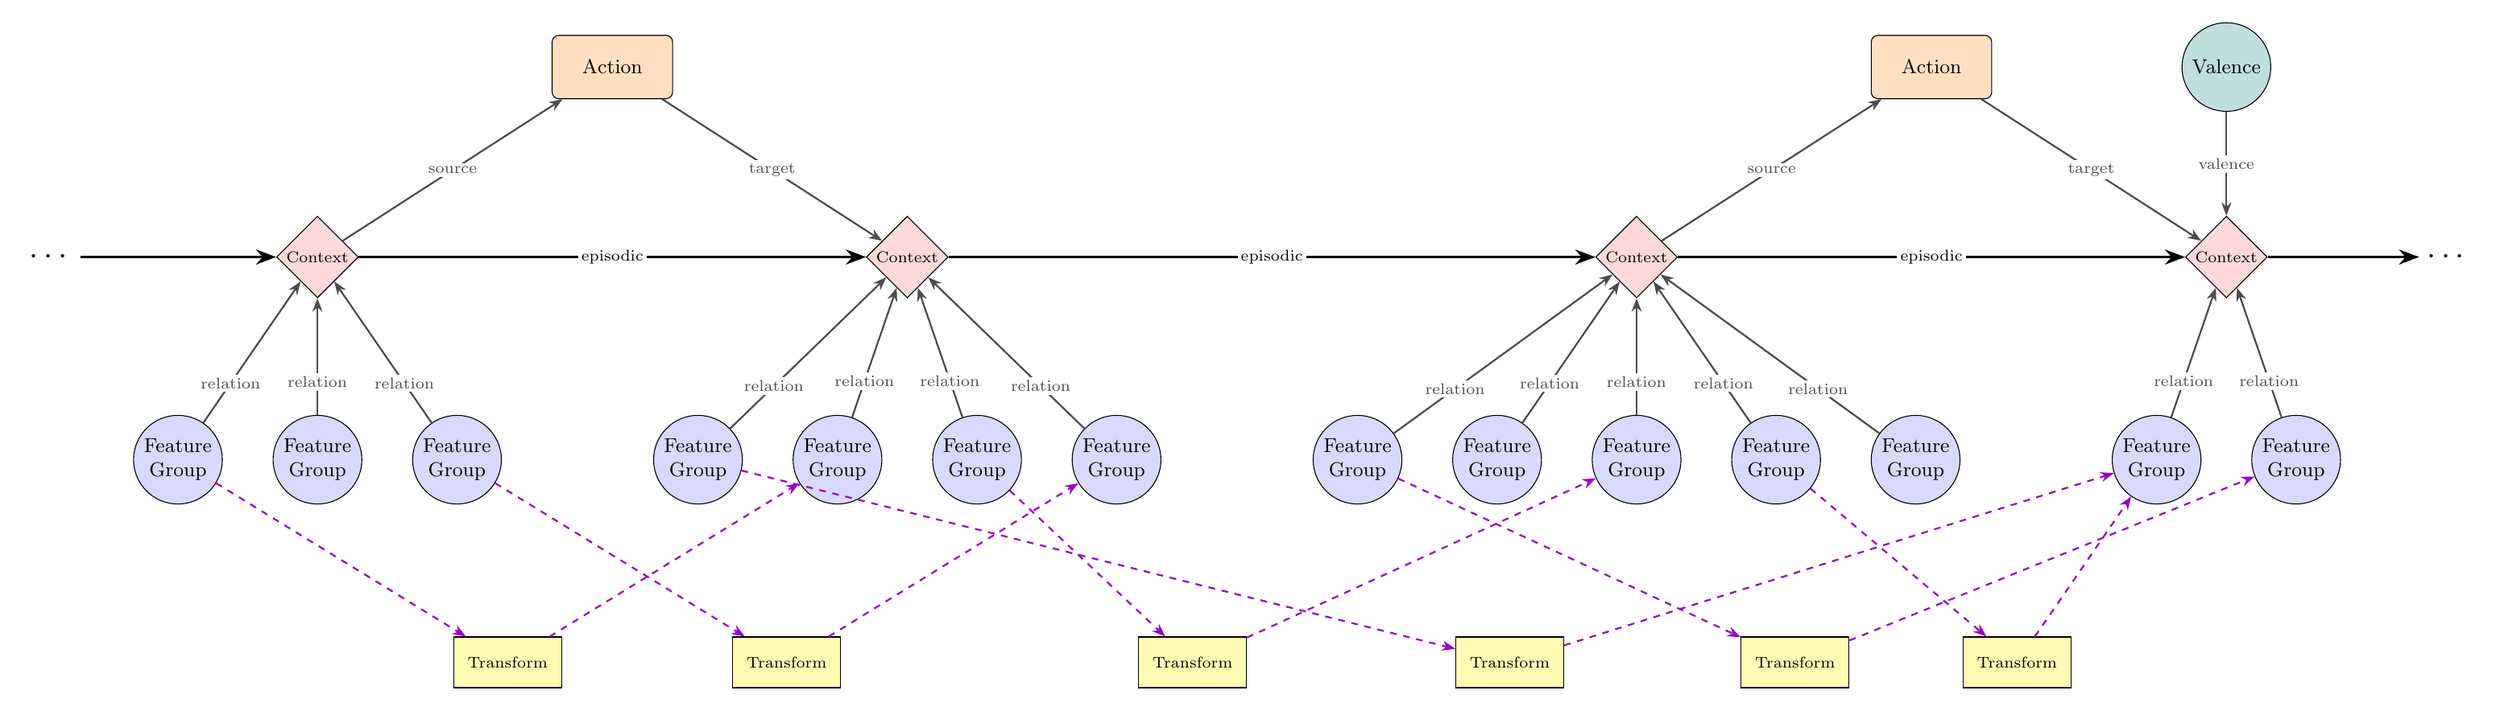
\begin{tikzpicture}[
    circ/.style={circle, draw, fill=featuregroup, minimum size=1.4cm, font=\small, align=center, inner sep=1pt},
    rel/.style={diamond, draw, fill=context, font=\scriptsize, align=center, inner sep=1pt},
    trans/.style={rectangle, draw, fill=transform, font=\scriptsize, align=center, inner sep=3pt, minimum height=0.8cm, minimum width=1.7cm},
    val/.style={circle, draw, fill=valence, minimum size=1.4cm, font=\small, align=center, inner sep=1pt},
    act/.style={rectangle, rounded corners=3pt, draw, fill=action, font=\small, align=center, inner sep=3pt, minimum height=1.0cm, minimum width=1.9cm},
    assoc/.style={-{Stealth[length=6pt]}, thick, color=black!70},
    epi/.style={-{Stealth[length=9pt]}, line width=1.1pt, color=black},
    tedge/.style={-{Stealth[length=6pt]}, thick, dashed, color=transformedge},
    lbl/.style={font=\scriptsize, fill=white, inner sep=1.5pt, align=center},
    x=1cm, y=1cm
  ]
    % feature groups (middle row)
    \node[circ] (fg1)  at (0,0)    {Feature\\Group};
    \node[circ] (fg2)  at (2.2,0)  {Feature\\Group};
    \node[circ] (fg3)  at (4.4,0)  {Feature\\Group};
    \node[circ] (fg4)  at (8.2,0)  {Feature\\Group};
    \node[circ] (fg5)  at (10.4,0) {Feature\\Group};
    \node[circ] (fg6)  at (12.6,0) {Feature\\Group};
    \node[circ] (fg7)  at (14.8,0) {Feature\\Group};
    \node[circ] (fg8)  at (18.6,0) {Feature\\Group};
    \node[circ] (fg9)  at (20.8,0) {Feature\\Group};
    \node[circ] (fg10) at (23.0,0) {Feature\\Group};
    \node[circ] (fg11) at (25.2,0) {Feature\\Group};
    \node[circ] (fg12) at (27.4,0) {Feature\\Group};
    \node[circ] (fg13) at (31.2,0) {Feature\\Group};
    \node[circ] (fg14) at (33.4,0) {Feature\\Group};

    % contexts (top row) on the episodic timeline
    \node[rel] (rg1) at (2.2,3.2)  {Context};
    \node[rel] (rg2) at (11.5,3.2) {Context};
    \node[rel] (rg3) at (23.0,3.2) {Context};
    \node[rel] (rg4) at (32.3,3.2) {Context};
    \node[font=\Large] (eb) at (-2.0,3.2) {$\cdots$};
    \node[font=\Large] (ea) at (35.8,3.2) {$\cdots$};

    % valence tag (only the right-most one is kept here)
    \node[val] (v3) at (32.3,6.2) {Valence};

    % actions (above the contexts, centered between the pair they connect)
    \node[act] (a1) at (6.85,6.2)  {Action};
    \node[act] (a2) at (27.65,6.2) {Action};

    % transforms (bottom row)
    \node[trans] (t1) at (5.2,-3.2)  {Transform};
    \node[trans] (t2) at (9.6,-3.2)  {Transform};
    \node[trans] (t3) at (16.0,-3.2) {Transform};
    \node[trans] (t4) at (21.0,-3.2) {Transform};
    \node[trans] (t5) at (25.5,-3.2) {Transform};
    \node[trans] (t6) at (29.0,-3.2) {Transform};

    % episodic timeline (thick before/after links)
    \draw[epi] (eb)  -- (rg1);
    \draw[epi] (rg1) -- (rg2) node[lbl, pos=0.5] {episodic};
    \draw[epi] (rg2) -- (rg3) node[lbl, pos=0.5] {episodic};
    \draw[epi] (rg3) -- (rg4) node[lbl, pos=0.5] {episodic};
    \draw[epi] (rg4) -- (ea);

    % relation edges: each Feature Group relates into its Context
    \draw[assoc] (fg1)  -- (rg1) node[lbl, pos=0.28] {relation};
    \draw[assoc] (fg2)  -- (rg1) node[lbl, pos=0.28] {relation};
    \draw[assoc] (fg3)  -- (rg1) node[lbl, pos=0.28] {relation};
    \draw[assoc] (fg4)  -- (rg2) node[lbl, pos=0.28] {relation};
    \draw[assoc] (fg5)  -- (rg2) node[lbl, pos=0.28] {relation};
    \draw[assoc] (fg6)  -- (rg2) node[lbl, pos=0.28] {relation};
    \draw[assoc] (fg7)  -- (rg2) node[lbl, pos=0.28] {relation};
    \draw[assoc] (fg8)  -- (rg3) node[lbl, pos=0.28] {relation};
    \draw[assoc] (fg9)  -- (rg3) node[lbl, pos=0.28] {relation};
    \draw[assoc] (fg10) -- (rg3) node[lbl, pos=0.28] {relation};
    \draw[assoc] (fg11) -- (rg3) node[lbl, pos=0.28] {relation};
    \draw[assoc] (fg12) -- (rg3) node[lbl, pos=0.28] {relation};
    \draw[assoc] (fg13) -- (rg4) node[lbl, pos=0.28] {relation};
    \draw[assoc] (fg14) -- (rg4) node[lbl, pos=0.28] {relation};

    % valence edge: the Valence node tags one Context
    \draw[assoc] (v3) -- (rg4) node[lbl, pos=0.5] {valence};

    % action edges: earlier Context -> Action -> later Context
    \draw[assoc] (rg1) -- (a1) node[lbl, pos=0.5] {source};
    \draw[assoc] (a1) -- (rg2) node[lbl, pos=0.5] {target};
    \draw[assoc] (rg3) -- (a2) node[lbl, pos=0.5] {source};
    \draw[assoc] (a2) -- (rg4) node[lbl, pos=0.5] {target};

    % transform edges: earlier Feature Group -> Transform -> later Feature Group
    \draw[tedge] (fg1)  -- (t1);  \draw[tedge] (t1) -- (fg5);
    \draw[tedge] (fg3)  -- (t2);  \draw[tedge] (t2) -- (fg7);
    \draw[tedge] (fg6)  -- (t3);  \draw[tedge] (t3) -- (fg10);
    \draw[tedge] (fg4)  -- (t4);  \draw[tedge] (t4) -- (fg13);
    \draw[tedge] (fg8)  -- (t5);  \draw[tedge] (t5) -- (fg14);
    \draw[tedge] (fg11) -- (t6);  \draw[tedge] (t6) -- (fg13);
  \end{tikzpicture}%
  }
  \caption{Action nodes are between Context nodes. Note that not every Context node is required to have an associated Action node.}
  \label{fig:action}
\end{figure}

\paragraph{Valence Selected Actions}
- Intrinsic valence (e.g. pain, hunger) creates problems for the agent that it must solve. In order to identify solutions to the problem, valence also acts as the index to potential solutions. The agent Simulates the path to the potential solutions and selects a satisficing option.
- Actions are not selected based on reward signals, they are selected for general homeostasis. Only if there is a problem (predicted threat, negative sensory valence due to hunger, etc.) will they seek out solutions using Option Generation and Simulation.

\paragraph{Habit Selected Actions}
- Actions are recorded with relation to the current context, enabling transference of actions to future scenarios with the same or similar context.
- Actions are selected based on Context: the actions that were taken previously in the given context are the actions that will be taken again.
- As the PresenceEdge of Actions trend towards certainty (i.e. ~1) they create scripts of actions (a/k/a "habits") based on strongly associated conceptual timelines

\paragraph{Option Generation}
- Indexes: concepts, timelines, valence
- "I'm hungry" -- find solutions to the problem through association; uses valence to find previous solutions
- Seeking out solutions to current problems is based on using Sensory Valence associated with the specific anticipated problem to identify options for solutions, then simulation to select options and potential paths to the options.

\subsection{Simulation}
- Contexts and transforms can be iterated through without taking actions to simulate situations
- (something) can create Contexts on the side that influence the path of the simulation so that the PresenceEdges followed in the simulation are not always the strongest edges
- Modified simulation: play through temporal links with modifications

\subsection{Introspection}
- Internal states must be available for observation to enable introspection
- Internal states that are available for introspection likely include confidence levels of prediction and simulation, recent memory, and recent perception -- basically the ability to inspect the recent episodic timeline.

\subsection{Future Work}
- Concepts and Contexts use many of the same structures and mechanisms (prediction monitors, abstraction, etc.). Can they be combined into a single structure? Or do they necessarily need to be separate.

\section{References}
\bibliographystyle{plainnat}
\bibliography{references}

\appendix
\section{Pseudocode}\label{sec:appx:a}

\subsection{Concepts}\label{pseudocode:concepts}

\subsection{Contexts}\label{pseudocode:contexts}

\subsection{Transforms}\label{pseudocode:transforms}
\begin{minted}{python}
class Transform:
    # the detected change between to Features or Relationships
    source: FeatureGroup
    target: FeatureGroup

    transforms: set[Delta]

class Delta:
    type: TransformType
    value: any

class TransformType(Enum):
    # an enumeration of the different types of transforms
    # this list is directly corresponding to the feature extractors
    # and the relationships that can be identified between concepts
    LOCATION = 1
    COLOR = 2
    DISTANCE = 3
    # ...
\end{minted}

\subsection{Edges}\label{pseudocode:edges}
\begin{minted}{python}
class Edge:
    # the Feature that the edge connects to
    # TODO: edges aren't just for features
    feature: Feature

    # Beta counts (present, absent)
    # presence_prob = a/(a+b) = criteriality
    a: int
    b: int

    # Normal-Gamma edge probability for continuous feature values (e.g. color)
    mu: float
    kappa: float
    alpha: float
    beta: float

    # Dirichlet edge probability for categorical feature values (e.g. up / down / left / right)
    # TODO: currently not used
    dir_counts: dict[any, int]  # count of features, any is the range of the feature the edge points to
    n: int

    def get_feature(self, features: FeatureGroup) -> Feature | None:
        # looks up the Feature that corresponds to the Feature expected by this Edge

    def probability_present(self) -> float:
        self.a / (self.a + self.b)

    # is this Edge present and of the right value in a set of Features
    # TODO: should be more than features
    def likelihood(self, features: FeatureGroup) -> float:
        present: bool = self.feature in features
    
        if not present:
            # expected but absent isn't a deal-breaker, maybe an occluded feature
            return(1 - self.probability_present())

        # calculate Student-t PDF for value
        val: float = self.get_feature(features).value
        value_term: float = scipy.stats.t(val, mu=self.mu, kappa=self.kappa, alpha=self.alpha, beta=self.beta)
    
        return value_term * self.probability_present()

    def update(self, features: FeatureGroup) -> None:
        present: bool = self.feature in features

        if not present:
            self.b += 1
            return

        # update presence counts
        self.a += 1
        self.n_raw += 1

        # sculpt edge value
        val: float = self.get_feature(features).value
        k = self.kappa
        mu_old = self.mu
        self.mu = (k * mu_old + x) / (k + 1)
        self.beta = self.beta + (k / (k + 1)) * (val - mu_old)^2 / 2
        self.kappa = k + 1
        edge.alpha = self.alpha + 0.5
\end{minted}

\subsection{Saliency}\label{pseudocode:saliency}
\begin{minted}{python}
def get_saliency_points():
    get_vision_saliency_points()
    get_aural_saliency_points()
    get_tactile_saliency_points()
    # etc.

    crossmodal_saliency_points()
\end{minted}

\begin{minted}{python}
def get_vision_saliency_points():
    feature_map = vision_feature_extractors()
\end{minted}

\subsection{Main Loop}\label{pseudocode:main-loop}
\begin{minted}{python}
def main():
    obs = get_observation()

    # --- 1. do feature extraction
    features = feature_extraction()

    # --- 2. get the salient features, bound together by location
    feature_groups = get_saliency_points(features)

    # --- 3. resolve previous prediction

    # --- 4. identify concepts
    concepts = identify_concepts(prev_context, feature_groups)

    # --- 5. identify context

    # --- 6. predict

    # --- 7. take action
\end{minted}

\section{Sufficiency Tests}
These are thought experiments to ensure that our cognitive architecture can (eventually) address the concerns below; however, it should be noted that the sufficiency tests are operating at a level of abstraction that wouldn't be initially available. Initially Concepts are operating at the Feature / FeatureGroup level -- which is pixels, waveforms, etc. These sufficiency tests presume that there have been multiple rounds of substantial acquisition and abstraction to create functional high-level concepts like "dog" and "cat" and "frisbee".

\subsection{A cat is not a dog}
- The agent has seen multiple dogs before of different varieties: roughly large, furry, four legged creatures, that pant, and are friendly. The agent encounters a new dog that generally meets the criteria of previous dogs, but has a few subtle differences such as pointier ears and whiskers. When the agent approaches the dog, it runs away which is counter to prediction. When the agent continues to pursue the dog it hisses and swipes its claws at the agent. This is not the behavior of previous dogs, it must be something new. A cat. 
- This is a demonstration of bifurcation of concepts based on different predictions of the objects.

\subsection{There's a bear in my kitchen}
- The agent enters the kitchen in a house -- a familiar scenario. There is a bear in the kitchen. The agent is able to recognize the bear without having encountered a bear in the kitchen before. 
- This is a demonstration of bottom-up recognition with incongruent context.

\subsection{Social Transfer}
- a child in a preschool is sitting with a teacher, the teacher holds up flashcards with different objects that are different colors. red car, blue car, red ball, yellow ball. the teacher asks the child the name of the color for each object, and the child learns how to recognize "red" objects and the meaning of the word "red".
- demonstrates social transfer from the teacher to the child, reification of concepts, and associating a word with a concept

\subsection{Emotion}
- \hl{TODO}
- happy, sad, disgust, fear, anger, surprise, shame, interest

\subsection{"Democracy"}
- A frequent challenge to grounded concepts is that they can't create the concept of "democracy" (as an example of a sufficiently abstract concept). Through iterative abstraction, grounded perceptual symbols would get further away from their grounding to create abstract symbols with no grounding. Specifically a high-level sketch of obtaining the concept of "democracy" would look something like:
	1. Learn the instance of "mother" as the one that is feeding the agent
	2. Learn the concept of "mothers" as other agents having a similar situation
	3. Experience "mothers" as setting and enforcing rules to create a concept of "authority figure"
	4. Learn through social transfer that there are different "authority figures", such as kings and presidents
	5. Learn that "kings" can be cruel and arbitrary and that fairness / equity / predictability is a desirable outcome
	6. Learn that people can vote to create equitable rules for the masses and that this is called "democracy"
    
\subsection{Language}
- Language is sounds and symbols tied to concepts, it has no special mechanisms.
- Sentence structure and grammar is learned by patterns.
- Symbol-to-concept binding is arbitrary – unlike feature-grounded concepts, a word shares no features with its referent.
- Language is also an input channel: create a token based on a sound or a set of symbols that needs to be filled in. It further gets associated with the relationships of words or concepts around it, based on explication, context clues, or assumption.
\subsection{Dog and Frisbee}
- A person throws a frisbee towards a dog. The agent is able to predict that the dog will chase towards the frisbee and whether or not it will be able to intercept it. 
- The prediction is not based on any reward signal and the agent has no reason to maintain a reward around dogs and frisbees.

\subsection{Stop signs don't matter when you are walking}
- when walking down the street, the agent barely notices stop signs and does not obey them
- when in a car, the agent notices stop signs through context-specific attention mechanisms
- demonstrates context-specific attention and saliency that leads to different contexts and actions

\subsection{The drapes are different in his memory}
- Legion season 1, they go back into the memory of Legion to his therapists office, then they visit the office in real life. The drapes have a different pattern in his memory than in real life.
- This is an example of episodic memory encoding rough concepts rather than precise feature group details.

\subsection{A handful of marbles}
- Agent has a memory of holding three marbles. In recollection it may recall the different colors and differentiation of size, but not the specific details of the patterns on the marbles. It will also recall the size of the marbles relative to each other and relative to the hand; the rough positioning in the hand; etc.
- This is an example of retaining some features in a feature group but eliminating others.

\subsection{Driving to work by mistake}
- You are running an errand on the weekend. The route you take starts by following the same route you always take to work, and then diverges part way through to the route you need to continue to run your errand. You accidentally miss your turn for your errand and continue driving to work.
- This is a demonstration of habits (strong association and strength of recall) dictating actions.

\subsection{Daydreaming}
- \hl{TODO}

\end{document}
